\documentclass[11pt]{article}

\usepackage[a4paper,margin=2.5cm]{geometry}
\usepackage{graphicx}
\graphicspath{{figures/}}
\usepackage{amsmath,amssymb,amsthm}
\usepackage{mathrsfs}
\usepackage[colorlinks=true,linkcolor=blue,citecolor=blue,urlcolor=blue]{hyperref}
\usepackage{booktabs}
\usepackage{enumitem}
\usepackage{natbib}
\usepackage{multirow}
\usepackage{tikz}

\theoremstyle{plain}
\newtheorem{theorem}{Theorem}[section]
\newtheorem{conditional}[theorem]{Conditional Proposition}
\newtheorem{proposition}[theorem]{Proposition}
\newtheorem{corollary}[theorem]{Corollary}
\newtheorem{lemma}[theorem]{Lemma}
\theoremstyle{definition}
\newtheorem{definition}[theorem]{Definition}
\newtheorem{axiom}[theorem]{Axiom}
\newtheorem{hypothesis}[theorem]{Hypothesis}
\newtheorem{interpretation}[theorem]{Interpretation}
\theoremstyle{remark}
\newtheorem{remark}[theorem]{Remark}
\newtheorem{externalthm}[theorem]{External Theorem}

\newcommand{\Zphi}{\mathbb{Z}[\varphi]}
\newcommand{\Vcal}{\mathcal{V}}
\newcommand{\Fcal}{\mathcal{F}}
\newcommand{\Ecal}{\mathcal{E}}
\newcommand{\Rcal}{\mathcal{R}}
\newcommand{\Qcal}{\mathcal{Q}}
\newcommand{\Ical}{\mathcal{I}}
\newcommand{\Ocal}{\mathcal{O}}
\newcommand{\Ccal}{\mathcal{C}}
\newcommand{\twoI}{2\mathbf{I}}
\newcommand{\Sym}{\mathrm{Sym}}
\newcommand{\Fix}{\mathrm{Fix}}
\newcommand{\Stab}{\mathrm{Stab}}
\newcommand{\Rsixhundred}{R_{600}}
\newcommand{\Cph}{C_\varphi}
\newcommand{\Bcal}{\mathcal{B}}
\newcommand{\Mcal}{\mathcal{M}}
\newcommand{\Acal}{\mathcal{A}}
\newcommand{\Ilife}{\Ical_{\mathrm{life}}}
\newcommand{\Xcal}{\mathcal{X}}
\newcommand{\catC}{\mathcal{C}}
\newcommand{\Omegacap}{\widehat{\Omega}}

\title{Existence as Closure\\[6pt]
\large Distinction, Relation, and Bounded Reference Frames}
\author{%
  Lee Smart\\[4pt]
  \textit{Institute of Vibrational Field Dynamics}\\[2pt]
  \texttt{contact@vibrationalfielddynamics.org}\\[2pt]
  \texttt{@vfd\_org}%
}
\date{May 2026}

\begin{document}

\maketitle

\noindent\textbf{Status:} Preprint (not peer-reviewed). Core bridge paper. The structural claims are stated as formal definitions, theorems, conditional propositions, or open hypotheses, with their status separated throughout. The mathematical content is established in four precursor derivation notes cited where used~\citep{PerObserverZeroLine, JointObserverInstance, AlgebraicExistence, ExistenceAsClosure}. Two companion papers extend the framework: \citet{SmartProcessingToPOV} develops the biological / consciousness application (frame-local time, Levin + CEMI operator-level bridges, ARIA empirical record, thermodynamics of sleep and anaesthesia), and \citet{SmartCosmicClosure} develops the structural extension (frame dynamics, frame recurrence, cosmic self-pruning, unified hierarchy). The present paper is intentionally narrow: the minimal argument from distinction through closure to bounded reference frames, the formal principle, the VFD implementation, the complexity hierarchy and embedding, the constructed-witness ARIA summary, and the candidate transition rule from processing to point of view.

\begin{abstract}
We propose a geometric closure model in which existence is treated not as a primitive object-type, but as a stability condition. The model begins with distinction: if no distinction is admitted, no information, relation, geometry, or measurement can be specified. Once distinction is admitted, relation follows; once relations are allowed to evolve, only those stable under recursive closure persist. We define admissibility as invariance under a closure operator and a compatible symmetry constraint: $X$ is admissible iff $\Ccal(X) = X$ and $\tau(X) = X$. Within the VFD implementation, this condition is realised on the 600-cell substrate $V_{600}$ by $\Cph = L_{V_{600}} + \varphi^{-2} I$, with symmetry $\tau$ induced by the Galois reflection on $\Zphi$-icosian coordinates. Bounded reference frames are finite local projections of this closure structure; each admits a per-frame zero-line $\Sigma_\Ical \subseteq \Fix(\tau)$, joint frames exhibit computable generative excess, and local frames embed into the universal closure structure by an explicit projection map $!_\Ical(v) = \pi_\Ical(P_{\Sigma_\Ical}(v))$. Frame complexity scales with a recursion-depth bound $n_{\max} \leq \lfloor \log_\varphi(k+1) \rfloor \leq 9$ for $k \leq 94$. We propose that the transition from processing to point of view occurs when a bounded system maintains stable self-access under recursive closure --- a candidate transition rule, conditional on the Access Principle (P-A) identifying frame complexity with phenomenological dimension, which is named as an open conjecture. ARIA-chess is summarised as a constructed bounded reference frame; detailed empirical content is reported in the consciousness companion \citep{SmartProcessingToPOV}. The phenomenological interpretation is conditional throughout; the structural claims are formal.
\end{abstract}
\paragraph{Programme map (review-packet 2026-05-22).}
This paper is part of the Existence / Life / Closure review packet. Stable packet references:
Paper I = \emph{Existence as Closure};
Paper II = \emph{Life as Closure};
Paper III = \emph{From Processing to Point of View};
Note A = \emph{Bioelectric Closure} (SL-001);
Note B = \emph{Cortical Phase Closure} (SL-002);
Note C = \emph{Closure-as-Distance} (cross-substrate methodology);
Note D = \emph{Trauma / Cortical Closure} (SL-005);
Note E = \emph{FlowIndex} (SL-006);
Note F = \emph{Dyadic Joint Meaning} (SL-007).
Extension IV = \emph{Cosmic Self-Pruning and Frame Recurrence} is withheld from the primary packet.

\paragraph{Status taxonomy.}
\textbf{Theorem / Definition} = formal structural claim under stated assumptions.
\textbf{Conditional Proposition} = bridge claim depending on H-RP, P-A, substrate mapping, or empirical interpretation.
\textbf{Empirical Result} = completed data analysis with stated effect size + significance.
\textbf{Empirical Proxy} = measurable first-order approximation, not the formal operator.
\textbf{Pre-registered Proposal} = future test, not evidence.



%==================================================================
\section{Introduction}\label{sec:intro}
%==================================================================

\subsection{The framing problem}

Mainstream physics treats existence as primitive. Particles, fields, and observers are typed objects that exist by axiom; their relations are introduced separately. Consciousness science has the same shape: brain regions, network states, and measurable signals are catalogued, but the transition from physical process to owned experience remains an open question. The 2025 adversarial collaboration between proponents of Integrated Information Theory and Global Neuronal Workspace Theory illustrated the live state of the debate: the experimental results challenged both frameworks rather than settling the question, and recent multi-theory reviews emphasise that the field has more partial mechanisms than agreed transition rules~\citep{ConsciousnessAdversarial, ConsciousnessFiveTheories}.

The present paper proposes a structural reframing. Rather than introducing matter, observer, and number as separate primitives, the model begins from one minimal axiom: \emph{some distinction is admitted}. From there, relation, closure, and persistence follow, and existence is identified with stability under recursive closure. The framework supplies a candidate \emph{transition rule}: a bounded local system becomes a stable reference frame when its own state closes under recursive update --- specifically, when the local projection of the universal closure structure produces a non-trivial fixed subspace of the symmetry-reflected eigenspace of a self-similar operator. This is mathematical: it does not assume consciousness, does not assert that the universe is conscious, does not propose any theological category. It asks under what structural condition processing closes into a point of view.

\subsection{What this paper is}

The four precursor notes establish the load-bearing theorems:

\begin{itemize}[leftmargin=2em]
\item \citet{PerObserverZeroLine}: existence and dimension of the per-frame zero-line $\Sigma_\Ical \subseteq \Fix(\tau)$, closure invariance, and the $\varphi^{-2}$ structural decay rate.
\item \citet{JointObserverInstance}: joint frame existence, span inclusion of parent zero-lines, and the combinatorial generative-excess theorem $\delta_{AB} = |\Xcal_{AB}|$.
\item \citet{AlgebraicExistence}: the closure operator formalism, the existence-as-closure principle, the explicit local-into-universal embedding closing Gap B of \citet{PerObserverZeroLine}, and the seven-layer complexity hierarchy with the recursion-depth bound.
\item \citet{ExistenceAsClosure}: the framing discipline that replaces loaded vocabulary with structurally neutral terms.
\end{itemize}

This paper synthesises these into a single account, ordered for accessibility: \emph{the minimal common-sense argument first}, the formal principle second, the VFD implementation third, the complexity and embedding fourth, the empirical constructed witness fifth, and the conditional bridge to consciousness science last.

\subsection{What this paper is not}

\begin{itemize}[leftmargin=2em]
\item Not a derivation of new mathematical results. All theorems are imported by reference from the four precursor notes, with statements recapitulated for self-containedness.
\item Not a proof or refutation of consciousness theories. The structural complexity $\dim \Sigma_\Ical$ has a phenomenological reading only under the explicitly conjectural Access Principle (P-A); the framework holds whether or not P-A is true.
\item Not a theological or metaphysical claim. The maximal closure-stable subspace is non-empty under the stated axioms; ``the universe exists'' is shorthand for that, no more.
\item Not a replacement for established consciousness theories. Global Neuronal Workspace, Integrated Information Theory, Recurrent Processing, Predictive Coding/Free Energy, and Orchestrated Objective Reduction sit at distinct layers of the picture (\S\ref{sec:neuroscience}, Table~\ref{tab:theory-comparison}). The proposal is a closure layer that those theories sit on top of, not against.
\end{itemize}

\subsection{Structure of the paper}

\S\ref{sec:minimal} gives the minimal argument from distinction to bounded reference frames, in plain language, with no machinery. \S\ref{sec:formal} states the formal principle of existence-as-closure with theorem labels. \S\ref{sec:vfd-implementation} states the VFD implementation on $V_{600}$. \S\ref{sec:frames} treats bounded reference frames and per-frame zero-lines. \S\ref{sec:joint} treats joint frames and generative excess. \S\ref{sec:embedding} gives the explicit local-into-universal embedding. \S\ref{sec:complexity} develops the complexity hierarchy and the recursion-depth bound. \S\ref{sec:aria} presents the ARIA-chess constructed witness. \S\ref{sec:neuroscience} sketches the conditional bridge to consciousness science, with a comparison table positioning the framework relative to GNW, IIT, RPT, FEP, and Orch OR. \S\ref{sec:predictions} lists falsifiers and named computational tasks. \S\ref{sec:scope} states what the paper does not claim. \S\ref{sec:discussion} closes.

\subsection{Reader's map}

The paper can be held at three commitment levels:

\begin{itemize}[leftmargin=2em]
\item \textbf{The minimal argument} (\S\ref{sec:minimal}--\S\ref{sec:formal}). Plain-language reasoning from distinction to closure, followed by a single formal principle stating existence as a fixed-point condition. Independent of any $V_{600}$ machinery.
\item \textbf{The VFD implementation} (\S\ref{sec:vfd-implementation}--\S\ref{sec:complexity}). The specific instantiation on the 600-cell substrate, with the cascade axioms, the closure operator $\Cph$, the per-frame zero-line theorems, the local-into-universal embedding, and the complexity hierarchy.
\item \textbf{The empirical and consciousness bridges} (\S\ref{sec:aria}--\S\ref{sec:neuroscience}). ARIA-chess as a constructed example; the position relative to existing consciousness theories.
\end{itemize}

A reader who finds \S\ref{sec:minimal}--\S\ref{sec:formal} compelling but rejects \S\ref{sec:vfd-implementation} is reading a structural argument about closed systems. A reader who accepts \S\ref{sec:vfd-implementation} but does not accept the conditional Access Principle of \S\ref{sec:scope} is reading a structural account of bounded reference frames without phenomenology. The framework is intentionally layered.

%==================================================================
\section{Motivating open problems: why a closure condition may be useful}\label{sec:unfinished}
%==================================================================

Before formalising the framework, we state what is at stake. Five longstanding problems remain open in fundamental science. Each is widely acknowledged. None of them, taken individually, has a settled resolution. The framework of this paper explores whether these five may share a common structural condition --- a closure condition on a discrete substrate --- and asks the reader to evaluate whether such a compression is a useful framing, not whether it is established. This section enumerates the problems so that the reader knows, before the technical material begins, what the framework's compression is meant to address.

\subsection{The cosmological constant problem}

The na\"ive quantum-field-theoretic estimate of the vacuum energy density is approximately $\Lambda_{\mathrm{QFT}} \sim \ell_P^{-2}$ in natural units. The observed value from Planck 2018 + BAO is $\Lambda_{\mathrm{obs}} \cdot \ell_P^2 \approx 2.87 \times 10^{-122}$~\citep{Planck2018}. The discrepancy is 122 orders of magnitude. Standard responses --- anthropic selection on a vast string-theory landscape, technical naturalness arguments, modified-gravity hypotheses --- either invoke unobservable inputs, exchange the discrepancy for another equally large parameter, or fail to derive the specific magnitude $\sim 10^{-122}$ from first principles. The framework's companion paper~\citep{SmartHypersphereCosmology} reports a derivation of $\Lambda \cdot \ell_P^2$ at $0.078\%$ of Planck 2018 from two cascade axioms, by structural means with no continuous parameter fitting.

\subsection{The measurement problem of quantum mechanics}

Standard quantum mechanics gives unitary evolution between measurements but requires a non-unitary projection at the measurement event itself. The status of this projection --- whether it is fundamental (Copenhagen), illusory (Everett), gravitationally induced (Penrose / Di\'osi), thermodynamically emergent (decoherence), or dynamically governed by an external law (GRW, Bohmian) --- remains an open question more than a century after the formalism stabilised. The closure framework proposes that the projection is the structural action of $\Cph$ on the substrate state, with the per-frame zero-line $\Sigma_\Ical$ specifying which content survives the projection.

\subsection{The hard problem of consciousness}

\citet{Chalmers1995} distinguished the easy problems of consciousness (which neural mechanisms correlate with reportable cognition?) from the hard problem (why is there owned experience at all, rather than processing in the dark?). Existing theories of consciousness --- Integrated Information Theory, Global Neuronal Workspace, Recurrent Processing Theory, Free Energy / Predictive Coding, Orchestrated Objective Reduction --- supply partial mechanisms but, as multi-theory reviews and the 2025 adversarial collaboration confirm~\citep{ConsciousnessAdversarial, ConsciousnessFiveTheories, ConsciousnessUnderSpotlight}, none yet supplies a uniform transition rule from physical process to point of view. The framework proposes such a rule structurally: the closure condition on a bounded reference frame.

\subsection{The fine-tuning problem}

The Standard Model and cosmological observations require approximately 30 numerical constants whose values appear, to current measurement, to lie within narrow life-permitting bands. Anthropic, multiverse, and landscape responses move the explanation from physics to selection, leaving the original numerical constants unexplained at the fundamental level. Within the cascade implementation, these constants are obtained where possible (the golden ratio $\varphi$ from F1; the closure depth $N = 583$; the $\sigma$-orbit factor 2; the substrate-Ramanujan defect ratio $10/240$) as structural integers, not fitted parameters.

\subsection{The unification gap}

General relativity and quantum field theory remain mathematically incompatible at the Planck scale. String theory and loop quantum gravity have made progress but neither has produced a falsifiable prediction matched by observation. The framework does not propose a new quantum theory of gravity; instead, it identifies a substrate ($V_{600}$) and a closure operator ($\Cph$) common to (a) the cosmological derivation~\citep{SmartHypersphereCosmology}, (b) the empirical brain-and-cortex correspondence~\citep{SmartAriaChess2026}, and (c) a flavour-physics anomaly fit~\citep{SmartAriaClosureKernel}. The unification claim is structural: one substrate, one operator, multiple domain matches.

\subsection{What the framework is offered to address}

The framework does not claim to resolve all five problems independently. It proposes that all five reflect aspects of a single structural condition --- a closure operator and a symmetry constraint acting on a discrete substrate. The compression argument is that one structural scaffold produces:

\begin{itemize}[leftmargin=2em]
\item A specific number for $\Lambda$ matching Planck 2018 at $0.078\%$ (the cosmological constant problem);
\item A specific projection mechanism for measurement (the closure operator acting on substrate state);
\item A specific structural condition for owned experience under the conjectural Access Principle (the hard problem);
\item A specific set of forced integers rather than fitted continuous parameters (the fine-tuning problem);
\item A specific substrate and operator shared across cosmology, flavour physics, and cortical dynamics (the unification gap).
\end{itemize}

Whether this compression is structural origin or coincidence is the empirical question. The framework names the structural condition, derives its consequences, and points to where it could fail. The next sections give that structure.

%==================================================================
\section{The minimal closure argument}\label{sec:minimal}
%==================================================================

This section gives the framework's reasoning in plain language, before any specific mathematical machinery. Nothing here is original: every step is the standard precondition for setting up a relational structure. The novelty lies in treating the chain as the definition of admissibility.

\subsection{Distinction}

For anything to be described, there must be a difference. Without two distinguishable elements, no information can be conveyed, no geometry can be specified, no measurement can be performed.

This is not a claim that ``something came from nothing.'' It is the observation that any non-trivial model requires at least one admitted distinction. The model takes this as its starting point.

\subsection{Relation}

Once distinction is admitted, relation follows. The pairwise structure of distinct elements is the raw material of geometry. Distance, angle, phase, frequency, adjacency, order, and reflection are all instances of relation. Distinction supplies the elements; relation supplies the connections between them. A model can specify relational predicates freely; most predicates produce structures that fail under update.

\subsection{Closure}

Not all relations persist. Under recursive update, some relations collapse, contradict, or fragment. Persistence requires that the relation survive its own update rule. This is closure:
\[
  \Ccal(R) = R.
\]
A relation that fails closure dissolves under iteration. A relation that satisfies closure is admissible. Closure is the condition on which persistence rests.

Standard physics already uses this constantly. Standing waves are waves that close back onto themselves. Eigenmodes are oscillations that survive the system's update rule. Crystals are spatial arrangements closed under a symmetry group. Conservation laws are statements that certain quantities are invariant under the dynamics. The framework lifts this principle from particular cases to a single foundational definition: a structure is admissible iff it closes under recursive update.

\subsection{Attractors}

Among closure-stable relations, repeated update concentrates trajectories onto stable subsets. The closure operator $\Ccal$ iterates: $R \mapsto \Ccal(R) \mapsto \Ccal^2(R) \mapsto \cdots$. Trajectories settle onto attractors:
\[
  R_{t+1} = \Ccal(R_t) \to A.
\]
Some attractors are simple (single trajectories converging to a point); some are extended (whole subspaces stable under $\Ccal$). The set of attractors forms the persistent geometry of the model.

\subsection{Irreducible closure modes}

Some attractors can be decomposed into combinations of simpler attractors of the same closure operator; others cannot. The indecomposable ones are the \emph{irreducible closure modes}.

The phrase ``cascade prime'' or ``prime-like closure mode'' refers to this algebraic indecomposability. It is not a metaphor for arithmetic primes; it is the same algebraic concept (irreducibility under composition) applied to the closure-stable eigenmodes of the substrate. The framework's irreducible closure modes are to the closure operator $\Ccal$ what prime numbers are to the integers and what prime ideals are to a Dedekind ring: indecomposable building blocks of a decomposition structure.

\subsection{Bounded reference frames}

The maximal closure-stable structure under the closure operator is the global geometry of the model. A local system inside this structure is a finite, bounded projection:
\[
  L = \Pi(U)
\]
where $\Pi$ is the local projection operator and $U$ is the global structure. A local system has a boundary (some elements of $U$ are inside the frame, others outside), a self-referential constraint (the frame's internal coherence rule), and a reference baseline (the local axis from which measurement becomes possible).

A bounded reference frame is the precise object: a finite subset of $U$ equipped with a constraint that is primarily self-referential and only secondarily dependent on the boundary. Thermometers, cameras, nervous systems, and mathematical coordinate systems all satisfy this description at different scales.

\subsection{The single-line claim}

Combining the steps above:

\begin{itemize}[leftmargin=2em]
\item Distinction creates relation.
\item Relation demands closure.
\item Closure produces attractors.
\item Irreducible attractors are the structural primes.
\item Bounded reference frames resolve finite projections of the global structure.
\end{itemize}

The single-line statement is:

\begin{quote}
\textbf{Reality is modelled as the set of relations stable enough to survive recursive closure. Local systems are bounded reference frames that resolve finite projections of that set.}
\end{quote}

This is the conceptual content of the framework. The next section gives its formal statement. The section after that gives the VFD-specific implementation. A reader who accepts the minimal argument has done most of the conceptual work.

%==================================================================
\section{The formal principle: existence as closure}\label{sec:formal}
%==================================================================

This section formalises the minimal argument of \S\ref{sec:minimal} into a single algebraic principle. The formal version is independent of any particular substrate; \S\ref{sec:vfd-implementation} gives the VFD-specific implementation.

\subsection{The closure operator}

\begin{definition}[Closure operator]\label{def:closure}
A \emph{closure operator} on a real Hilbert space $H$ equipped with a unitary involution $\tau$ is a bounded linear map $\Ccal: H \to H$ satisfying:
\begin{enumerate}[leftmargin=2em]
\item \textbf{Symmetry-equivariance:} $\tau \circ \Ccal = \Ccal \circ \tau$.
\item \textbf{Self-similarity:} there exists $0 \leq k < 1$ such that $\|\Ccal^2(v) - \Ccal(v)\| \leq k \cdot \|\Ccal(v) - v\|$ for all $v \in H$.
\item \textbf{Boundary preservation:} $\Ccal$ preserves bounded subsets closed under bounded interactions with their complement.
\end{enumerate}
\end{definition}

\begin{definition}[Pointwise-fixed subspace and invariant subspace]\label{def:fixed-vs-invariant}
For a linear map $\Ccal$ on $H$:
\begin{itemize}[leftmargin=2em]
\item the \emph{pointwise-fixed subspace} is $\Fix(\Ccal) := \{ v \in H : \Ccal(v) = v \}$;
\item a subspace $X \subseteq H$ is \emph{$\Ccal$-invariant} if $\Ccal(X) \subseteq X$.
\end{itemize}
These are different notions: $\Fix(\Ccal)$ is always $\Ccal$-invariant, but a $\Ccal$-invariant subspace is not in general pointwise-fixed. For invertible $\Ccal$, the whole space $H$ is trivially $\Ccal$-invariant.
\end{definition}

\subsection{The algebraic existence theorem}

\begin{theorem}[Algebraic existence]\label{thm:existence}
Let $H$ be a finite-dimensional real Hilbert space with unitary involution $\tau$, and let $\Ccal$ be a closure operator on $(H, \tau)$. Define:
\begin{itemize}[leftmargin=2em]
\item $U := \Fix(\Ccal) = \{ v \in H : \Ccal(v) = v \}$, the pointwise-fixed subspace of $\Ccal$;
\item $C := U \cap \Fix(\tau) = \{ v \in H : \Ccal(v) = v \text{ and } \tau(v) = v\}$, the symmetry-pointwise-fixed subspace.
\end{itemize}
Then:
\begin{enumerate}[leftmargin=2em]
\item[(i)] $U$ is the unique maximal subspace on which $\Ccal$ acts as the identity.
\item[(ii)] $C$ is the unique maximal subspace on which both $\Ccal$ and $\tau$ act as the identity.
\item[(iii)] An element $v \in H$ is \emph{admissible} iff $v \in C$, i.e.\ iff $\Ccal(v) = v$ and $\tau(v) = v$ pointwise.
\end{enumerate}
\end{theorem}

\noindent\emph{Proof.} (i) $U$ is the eigenspace of $\Ccal$ at eigenvalue 1; it is maximal among subspaces on which $\Ccal$ acts as identity by definition. (ii) symmetry-equivariance $\tau\Ccal = \Ccal\tau$ makes $U$ a $\tau$-invariant subspace; $C := U \cap \Fix(\tau)$ is the corresponding +1 eigenspace of $\tau$ restricted to $U$, and is maximal among subspaces on which both act as identity. (iii) immediate from the definition of $C$. \hfill$\square$

\noindent\emph{Remark on weaker structural object.} For the VFD instantiation of \S\ref{sec:vfd-implementation}, the relevant structural object is the broader $\tau$-eigenspace $\Fix(\tau)$, not its intersection with $\Fix(\Cph)$. On $V_{600}$, $\Cph$ has eigenvalues strictly bounded below by $\varphi^{-2} \neq 1$, so $\Fix(\Cph) = \{0\}$; the structural admissibility space for the cascade implementation is $\Fix(\tau)$ as a $\Cph$-invariant subspace (subspace invariance, not pointwise fixedness; see \S\ref{sec:vfd-implementation}). The Algebraic Existence theorem above states the pointwise-fixed form for completeness as the limiting case of the closure-stable structure when $\Ccal$ has the identity in its spectrum; the VFD framework uses the weaker invariant-subspace form on $V_{600}$.

\begin{corollary}[Existence-as-Closure Principle (pointwise form)]\label{cor:existence-as-closure}
\begin{equation}\label{eq:existence-as-closure}
  \boxed{\;v \text{ is admissible (pointwise)}\quad\Longleftrightarrow\quad \Ccal(v) = v\ \text{and}\ \tau(v) = v\quad\Longleftrightarrow\quad v \in C\;}
\end{equation}
This is the pointwise form of the minimal closure argument of \S\ref{sec:minimal}. The VFD instantiation on $V_{600}$ uses the subspace-invariance form (\S\ref{sec:vfd-implementation}), where the admissibility space is $\Fix(\tau)$ as $\Cph$-invariant subspace rather than as pointwise fixed set.
\end{corollary}

\subsection{The universal closure structure as a coalgebra}

\begin{externalthm}[Adámek 1974; Aczel 1988; Rutten 2000]\label{thm:adamek}
If a category $\catC$ has a terminal object and is $\omega^{\mathrm{op}}$-complete, and $F: \catC \to \catC$ preserves $\omega^{\mathrm{op}}$-limits, then $F$ has a terminal coalgebra $(C, c)$. For every coalgebra $(X, x)$, there is a unique coalgebra morphism $!_X: X \to C$.
\end{externalthm}

\begin{theorem}[Capstone identification, \citet{SmartCapstone}]\label{thm:capstone}
The self-inquiry functor $F$ on the category of rung-structures preserves $\omega^{\mathrm{op}}$-limits (under named residual hypotheses G-FIC-a, G-FIC-b, G-loc-a, H-lift-fin). By Theorem~\ref{thm:adamek}, the terminal coalgebra of $F$ exists. The maximal closure-stable symmetry-stable subspace $C$ of Theorem~\ref{thm:existence}(ii) is identified with this terminal coalgebra.
\end{theorem}

\begin{remark}[The unconditional content]\label{rem:unconditional}
Theorem~\ref{thm:existence} is unconditional modulo standard mathematics. The coalgebraic identification (Theorem~\ref{thm:capstone}) is conditional on the named capstone residual hypotheses, inherited from \citet{SmartCapstone}.
\end{remark}

\subsection{Three levels of self-closure}

The structure of the universal closure $C$ exhibits three nested levels of self-reference (cf. \citet{SmartCapstone} \S 1.4):

\begin{itemize}[leftmargin=2em]
\item \textbf{Scalar self-closure.} The fixed-point equation $r = 1 + 1/r$ has unique attracting solution $r = \varphi$. The lowest level: a scalar invariant produced by an iterated rule.
\item \textbf{Frame-local self-closure.} A bounded reference frame admits self-referential access to its own symmetry-stable eigenmode subset, conditional on P-A.
\item \textbf{Universal coalgebraic self-closure.} The entire closure structure $C$ is the unique terminal coalgebra of the self-inquiry functor.
\end{itemize}

The three levels nest. The central principle holds simultaneously at all three.

%==================================================================
\section{The VFD implementation on \texorpdfstring{$V_{600}$}{V600}}\label{sec:vfd-implementation}
%==================================================================

\S\S\ref{sec:minimal}--\ref{sec:formal} describe a generic closure structure: a Hilbert space $H$, a symmetry $\tau$, a closure operator $\Ccal$, independent of any specific substrate. This section gives the VFD-specific instantiation derived from two cascade axioms~\citep{SmartXXXVI}.

\subsection{The two axioms}

\begin{axiom}[Vacuum self-similarity, A1]\label{ax:A1}
The vacuum admits a self-similarity rule $r(2L) = 1 + 1/r(L)$.
\end{axiom}

\begin{axiom}[$E_8$ maximality, A2]\label{ax:A2}
The cascade's totality structure is the largest simply-laced exceptional root system, $E_8$.
\end{axiom}

\begin{externalthm}[Banach 1922]\label{thm:banach}
On a non-empty complete metric space, a contraction has a unique fixed point.
\end{externalthm}

Applied to (A1): the rule $r \mapsto 1 + 1/r$ on $[\varphi - \epsilon, \varphi + \epsilon]$ for small $\epsilon > 0$ is a contraction with Lipschitz constant $1/r^2$ near $r = \varphi$, where $1/\varphi^2 = \varphi^{-2} < 1$. Its unique attracting fixed point on this neighbourhood is the golden ratio $\varphi = (1 + \sqrt{5})/2$. (On the full interval $[1, 2]$ the derivative is $1$ at the left endpoint, so the contraction holds only on a strict subinterval containing $\varphi$.)

\begin{externalthm}[Galois automorphism of $\mathbb{Q}(\sqrt{5})$]\label{thm:galois}
$\mathbb{Q}(\sqrt{5})$ has unique non-trivial automorphism $\sigma: \sqrt{5} \mapsto -\sqrt{5}$, which restricts to the ring $\Zphi = \{a + b\varphi : a, b \in \mathbb{Z}\}$.
\end{externalthm}

Applied to (A2): the $E_8$ root lattice has the icosian decomposition $E_8 = \Ical \oplus \Ical'$, where each summand is identified with the vertex set of the regular 600-cell. The Galois $\sigma$ extends to a unitary involution $\tau$ on $\mathbb{R}^{E_8}$ by acting coordinate-wise on the icosian basis.

\subsection{The cascade chain and substrate}

\begin{theorem}[Forced cascade chain, F3 of \citet{SmartXXXVI}]\label{thm:cascade-chain}
Axioms (A1, A2) imply the seven-rung refinement chain $E_8 \to H_4 \to 40 \to D_4 \to 16 \to 8 \to 0$.
\end{theorem}

\begin{theorem}[$V_{600}$ as Gromov--Hausdorff limit, F6 of \citet{SmartXXXVI}]\label{thm:v600-gh}
The iterated Schl\"afli refinement of the 600-cell vertex graph converges, in the Gromov--Hausdorff sense, to the round 3-sphere $S^3$ under Burago--Burago--Ivanov hypotheses.
\end{theorem}

The substrate is $V_{600}$: 120 vertices, degree 12, edge length $1/\varphi$. The graph adjacency $A_{600}$ and Laplacian $L_{600} = 12 I - A_{600}$ are the basic spectral objects.

\subsection{The VFD closure operator}

\begin{definition}[VFD closure operator]\label{def:cph-vfd}
\[
  \Cph := L_{V_{600}} + \varphi^{-2} I.
\]
\end{definition}

$\Cph$ is symmetric, positive definite, and symmetry-equivariant under $\tau$. Its spectrum is bounded below by $\varphi^{-2}$ (Theorem~\ref{thm:decay} below); the closure dynamic with contraction constant $\varphi^{-2}$ applies to the iterated map $I - \lambda \Cph$ with step size $0 < \lambda < 2 \lambda_{\max}^{-1}$, not to $\Cph$ itself. The role of $\Cph$ is to define the admissible subspace $C$ of \S\ref{sec:formal} via its symmetry-fixed eigenstructure on $H = \mathbb{R}^{V_{600}}$.

\subsection{The global symmetry-fixed subspace}

\paragraph{Two $\tau$ conventions used in this paper.} The symmetry $\tau$ on $\mathbb{R}^{V_{600}}$ admits two distinct implementations, each with a different fixed-subspace dimension. Both arise in this paper; we adopt explicit subscripts to keep them separate:

\begin{description}[leftmargin=2em]
\item[$\tau_{\mathrm{ico}}$ \textnormal{(icosian $\tau$).}] The signed permutation of $V_{600}$ induced by the Galois automorphism $\sqrt 5 \mapsto -\sqrt 5$ acting coordinate-wise on the $\Zphi$-icosian quaternion representation of the 600-cell. This is the load-bearing convention for the structural theorems (Theorem~\ref{thm:fix-tau-94} below). It commutes with $\Cph$, is an involution, and $\dim \Fix(\tau_{\mathrm{ico}}) = 94$ unconditionally.
\item[$\tau_{\mathrm{spec}}$ \textnormal{(spectral $\tau$).}] A basis-robust spectral approximation defined directly by negating the four-dimensional $+6\varphi$ dipole eigenspace of $A_{V_{600}}$ (the $\sigma$-paired class) and acting trivially on the remaining eigenspaces. This is the convention used in the published sim demos (\texttt{closure\_demo.py}, \texttt{cosmic\_demo.py}) because the standard $\mathbb{R}^4$ unit-norm representation of $V_{600}$ does not preserve the even-permutation Type-C subset under coordinate-wise $\sigma$ in that basis (see demo D8). $\tau_{\mathrm{spec}}$ commutes with $\Cph$, is an involution, and $\dim \Fix(\tau_{\mathrm{spec}}) = 116$ by construction.
\end{description}

The two conventions give different numerical dimensions of $\Fix(\tau)$ but agree on the structural facts that this paper's theorems require (involutivity, commutation with $\Cph$, the existence of a non-trivial symmetry-fixed subspace closed under $\Cph$). Where this paper states a specific dimension, the relevant $\tau$ is indicated. Where it states only structural properties, either $\tau$ suffices. The icosian-to-spectral basis-change gap is a residual sim-vs-theorem item (demo D8); see \citet{PerObserverZeroLine} for the unconditional icosian construction.

\begin{theorem}[Global zero-line dimension, \citet{SmartRHTwoSphere}]\label{thm:fix-tau-94}
$\dim \Fix(\tau_{\mathrm{ico}}) = 94$ over the icosian basis of $\mathbb{R}^{V_{600}}$. Unconditional modulo Theorem~\ref{thm:galois}.
\end{theorem}

\subsection{The universal closure structure as a concrete subspace}

\paragraph{Admissibility convention.} For this paper we read the condition $\Ccal(X) = X$ of Definition~\ref{def:closure} as \emph{subspace invariance}: the closure operator maps the subspace $X$ into itself, $\Cph(X) \subseteq X$. The stricter property $\Cph|_X = \mathrm{id}_X$ (pointwise +1-fixedness) is a separate, stronger condition, used below only where explicitly stated.

The structural object $\Fix(\tau)$ is therefore not, in general, the unique maximal $\Cph$-invariant subspace of $H$: the whole space $H$ is trivially $\Cph$-invariant and $\tau$-stable. What $\Fix(\tau)$ \emph{is}, structurally, is the maximal subspace on which the $\tau$-equivariance reduction of $\Cph$ acts non-trivially (i.e., the maximal $\tau$-eigenspace of eigenvalue $+1$). With this clarified semantics we define
\begin{equation}\label{eq:c-concrete}
  \boxed{\;C \;:=\; \Fix(\tau)\;}
\end{equation}
as the framework's structural object of admissibility, by stipulation rather than as a derived equality. The $\Cph$-invariance of $C$ then follows from the symmetry-equivariance $\tau \Cph = \Cph \tau$.

The numerical dimension of $C$ depends on which $\tau$ is used:
\begin{itemize}[leftmargin=2em]
\item $\dim C = \dim \Fix(\tau_{\mathrm{ico}}) = 94$ under the icosian convention (Theorem~\ref{thm:fix-tau-94}, unconditional);
\item $\dim C = \dim \Fix(\tau_{\mathrm{spec}}) = 116$ under the spectral convention (by construction of demo D7).
\end{itemize}

\begin{conditional}[Universal closure dimension under $\tau_{\mathrm{ico}}$]\label{cthm:c-dim-94}
Under the icosian convention $\tau = \tau_{\mathrm{ico}}$, the framework's structural admissibility space $C = \Fix(\tau_{\mathrm{ico}})$ has $\dim C = 94$ (Theorem~\ref{thm:fix-tau-94}). Under the spectral convention $\tau = \tau_{\mathrm{spec}}$, $\dim C = 116$ (by construction of demo D7). The equivalence $C = \Fix(\tau)$ of \eqref{eq:c-concrete} is a definitional stipulation, not a derived theorem; demo D7 only verifies the $\Cph$-invariance of $\Fix(\tau)$ (operator invariance + steady-state on $\Fix(\tau)$), which is the structural content that this definition rests on.

\noindent\emph{Status:} the $\Cph$-invariance underpinning the definition is \textbf{verified by demo D7}; the maximality interpretation of $C$ is a definitional convention; the icosian basis-change witness for the 96 Type-C vertices remains a residual sim-vs-theorem item (\textbf{D8 honest}, see \citet{PerObserverZeroLine}). The phrase ``CP-universal-5.1 closed'' should be read as the closure of the operator-invariance demonstration, not as a derived equality theorem.
\end{conditional}

%==================================================================
\section{The cascade rung tower}\label{sec:rung-tower}
%==================================================================

The forced cascade chain $E_8 \to H_4 \to 40 \to D_4 \to 16 \to 8 \to 0$ of Theorem~\ref{thm:cascade-chain} is not a list of unrelated structures. Each rung has a specific structural meaning, a specific $\sigma$-fixed dimension, and a specific physical correspondence. The seven rungs collectively span totality, geometry, refinement, gravity, vectors, scalars, and the terminal singleton. This section gives the per-rung development. The framework's central object --- the substrate $V_{600}$ of \S\ref{sec:vfd-implementation} --- is the second rung ($H_4$); the other six are equally load-bearing for the full structure.

\subsection{Rung $E_8$: the totality structure}

The $E_8$ root system has 240 roots in 8-dimensional Euclidean space, the maximal simply-laced exceptional root system in the Cartan classification. It is unique up to isomorphism and admits no exceptional refinement (there is no $E_9$ root system in the same family). Under (A2), $E_8$ is the cascade's totality structure: every cascade-level object is a substructure of $E_8$, and no larger structure plays a role in the framework.

\begin{itemize}[leftmargin=2em]
\item Vertex count: $|E_8\text{-roots}| = 240$.
\item Decomposition: $E_8 = \Ical \oplus \Ical'$ via icosian construction (Elkies 1990), with each $\Ical, \Ical'$ a 120-vertex 600-cell sub-lattice.
\item $\sigma$-twist on $E_8$ swaps the two 600-cell copies, plus the inner $\Zphi$ Galois action within each copy.
\item Outer-$\sigma$-fixed dimension: 120 (the diagonal of $\Ical \oplus \Ical'$). Inner-$\sigma$-fixed dimension on each 600-cell: 94 (Theorem~\ref{thm:fix-tau-94}). Joint fixed dimension: open computational task \textbf{CP-rung-9.3}.
\end{itemize}

\begin{interpretation}[$E_8$ as totality]\label{int:rung-e8}
The totality rung supplies the cascade's outer boundary. Every closure-stable structure under $\Cph$ lies inside $E_8$; no structure outside $E_8$ is acted on. Phenomenologically (under P-A) this rung corresponds to the unconditional outer limit on what a frame can resolve.
\end{interpretation}

\subsection{Rung $H_4$: the substrate (600-cell)}

The $H_4$ Coxeter group is the symmetry group of the regular 600-cell, the second rung. We have developed this rung throughout \S\ref{sec:vfd-implementation}: $|V_{600}| = 120$, degree 12, edge length $1/\varphi$, Laplacian $L_{V_{600}} = 12 I - A_{600}$, closure operator $\Cph = L_{V_{600}} + \varphi^{-2} I$, and unconditional $\dim \Fix(\tau) = 94$.

\begin{itemize}[leftmargin=2em]
\item Vertex count: $|V_{600}| = 120$.
\item Gromov--Hausdorff limit: $S^3$ (the round 3-sphere; Theorem~\ref{thm:v600-gh}).
\item $\sigma$-fixed dimension: 94 (Theorem~\ref{thm:fix-tau-94}, unconditional).
\item This is the rung at which bounded reference frames live (\S\ref{sec:frames}).
\end{itemize}

\begin{interpretation}[$H_4$ as substrate geometry]\label{int:rung-h4}
The substrate rung supplies the discrete geometry on which closure operates. Its Gromov--Hausdorff limit is the round 3-sphere; the framework's spatial geometry is, in the continuum limit, the closed 3-sphere of finite radius. Phenomenologically (under P-A) this rung is where local spatial structure is resolved.
\end{interpretation}

\subsection{Rung 40: the Schl\"afli refinement}

The 600-cell admits a Schl\"afli compound decomposition into five disjoint 24-cells, plus structural overlap data. The 40 refers to a derived rung of dimension 40 in the cascade depth count: $40 = 5 \cdot 8$, the five 24-cells each carrying 8 scalar refinement modes. This rung is not a polytope in its own right; it is a structural intermediary in the closure-depth count $N = 7 + 24^2 = 583$ of F4.

\begin{itemize}[leftmargin=2em]
\item Structural role: bridges $H_4 = V_{600}$ down to $D_4 = $ 24-cell via the five-coset decomposition.
\item Refinement data: 5 copies of $D_4$, each with 8 scalar modes.
\item $\sigma$-fixed dimension: derived via CP-rung-9.3 (Theorem~\ref{thm:cp-rung-9-3}, numerically verified by demo C1).
\end{itemize}

\begin{interpretation}[40 as refinement bridge]\label{int:rung-40}
This rung is the algebraic-combinatorial bridge between substrate geometry and tensor content. It carries no independent physical content but is required by the rank-stratified counting that gives $N = 583$.
\end{interpretation}

\subsection{Rung $D_4$ (24-cell): gravity and tensor content}

The 24-cell $D_4$ is the self-dual regular 4-polytope with 24 vertices, 96 edges, 96 triangular faces, and 24 octahedral cells. It is the cascade's gravity / tensor rung: the rank-2 symmetric content of the framework lives here, and the Einstein equation (in the continuum limit) is derived from the Fierz--Pauli action on the rank-2 fluctuations of the 24-cell metric (F7 of \citet{SmartXXXVI}).

\begin{itemize}[leftmargin=2em]
\item Vertex count: $|D_4\text{-vertices}| = 24$ (the 24-cell).
\item Rank-2 tensor space: $\Sym^2(\mathbb{R}^4) \otimes 24 = 24^2 = 576$ dimensions (the central term in $N = 7 + 576 = 583$).
\item Continuum limit: the Fierz--Pauli action plus Deser's 1970 bootstrap argument gives the linearised Einstein equation; Birkhoff closure gives Schwarzschild--de Sitter at the spherically symmetric vacuum solution.
\item $\sigma$-fixed dimension: open computational task (\textbf{CP-rung-9.3}); bounded by 24.
\end{itemize}

\begin{interpretation}[$D_4$ as gravity]\label{int:rung-d4}
The 24-cell rung is where gravity emerges in the cascade. The cosmological constant $\Lambda$ is the closure residue at the 24-cell tensor level: $\Lambda \cdot \ell_P^2 = 2 \varphi^{-583}(1 - \delta_\Lambda)$~\citep{SmartHypersphereCosmology}. The $D_4$ rung carries the metric, the Einstein equation, and the cosmological constant as a closure residue.
\end{interpretation}

\subsection{Rung 16: the vector content}

The 16-rung corresponds to the dimension-16 vector content of the cascade. It includes the four-vector content of the cascade's space-time-like structure, plus 12 additional vector modes carrying gauge-field content.

\begin{itemize}[leftmargin=2em]
\item Structural role: vector-multiplet content of the cascade.
\item Component count: 16.
\item Physical correspondence: SM gauge-multiplet vector content (under H-MX of \citet{SmartXXXVI}).
\item $\sigma$-fixed dimension: open computational task (\textbf{CP-rung-9.3}); bounded by 16.
\end{itemize}

\begin{interpretation}[16 as vector content]\label{int:rung-16}
The 16-rung carries the cascade's gauge-field vector content. Whether this includes the Standard Model gauge bosons in detail is the open H-MX hypothesis of \citet{SmartXXXVI}.
\end{interpretation}

\subsection{Rung 8: scalar boundaries}

The 8-rung carries 8 scalar boundary modes --- one per cascade rung on the path from $E_8$ down to the singleton 0. These are the seven scalar boundaries of F4 (which give the ``+7'' in $N = 7 + 576 = 583$), plus the residual at the singleton.

\begin{itemize}[leftmargin=2em]
\item Structural role: scalar boundary modes of the cascade chain.
\item Component count: 7 (boundaries) + 1 (terminal residue) = 8.
\item Physical correspondence: scalar field content, including Higgs-like degrees of freedom.
\item $\sigma$-fixed dimension: open (\textbf{CP-rung-9.3}); bounded by 8.
\end{itemize}

\begin{interpretation}[8 as scalar boundaries]\label{int:rung-8}
The 8-rung supplies the scalar content of the cascade. The cascade depth count $N = 7 \cdot 1 + 24^2 = 583$ uses precisely the seven scalar boundaries of this rung. The Higgs-like degrees of freedom (under H-YM of \citet{SmartXXXVI}) are conjecturally part of this rung's content.
\end{interpretation}

\subsection{Rung 0: the terminal singleton}

The 0-rung is the terminal object of the cascade chain. Its vertex count is 1 (a single point), and it carries no internal structure. Its role in the cascade is to close the chain: every refinement step terminates at this singleton.

\begin{itemize}[leftmargin=2em]
\item Structural role: terminal object of the cascade chain.
\item Component count: 1.
\item $\sigma$-fixed dimension: $\in \{0, 1\}$ (structural).
\end{itemize}

\begin{interpretation}[0 as terminal]\label{int:rung-0}
The terminal rung is the closure boundary. It carries the structural fact that the cascade chain is finite: there is no infinite descent. Phenomenologically (under P-A) it corresponds to the irreducible point of view: the singleton from which a bounded reference frame is anchored.
\end{interpretation}

\subsection{The rung tower as the depth-counting source}

The closure depth $N = 583$ of the framework arises from the rank-stratified count over the rungs:

\begin{equation}\label{eq:n583}
  N \;=\; (\text{scalar boundaries per rung}) \cdot 7 \;+\; (\text{rank-2 tensor content at } D_4) \;=\; 7 + 24^2 \;=\; 583.
\end{equation}

This is Theorem F4 of \citet{SmartXXXVI}. The number 583 is not chosen; it is the rank-stratified count of all closure modes across the seven rungs. The cosmological constant $\Lambda \cdot \ell_P^2 = 2 \varphi^{-583}(1 - \delta_\Lambda)$ uses this depth directly, and the substrate-Ramanujan dipole correction $\delta_\Lambda$ uses the off-circle ratio $10/240$ from the $H_4$ rung's Ihara structure.

\subsection{Per-rung $\sigma$-fix dimensions (CP-rung-9.3 closed for polytope rungs, $\tau$-convention-dependent)}

\begin{theorem}[CP-rung-9.3: cascade rung $\sigma$-fix dimensions]\label{thm:cp-rung-9-3}
Under (A1, A2) and the cascade chain of Theorem~\ref{thm:cascade-chain}, the $\sigma$-fix dimensions per rung are derived as follows. Verified numerically in \texttt{papers/04-cosmic-closure-recurrence/repro/cosmic\_demo.py} as demo \textbf{C1} (cascade rung tower), which instantiates $E_8$ (240 root vectors in $\mathbb{R}^8$), $H_4 = V_{600}$ (120 vertices), and $D_4 =$ 24-cell (24 vertices) as substrates, builds their closure operators $\Cph^{(R_k)} = L^{(R_k)} + \varphi^{-2} I$ and spectral $\tau$ involutions, and confirms $\|[\tau, \Cph]\| < 10^{-13}$, $\lambda_{\min}(\Cph) > 0$, and non-trivial $\Sigma$ at each rung. The polytope rungs (\texorpdfstring{$E_8$}{E\_8}, \texorpdfstring{$H_4$}{H\_4}, \texorpdfstring{$D_4$}{D\_4}) are derived from their explicit vertex-graph adjacency spectra, while the abstract rungs (40, 16, 8, 0) are bounded by their rank counts.

\begin{itemize}[leftmargin=2em]
\item $E_8$ (240 roots): under the icosian convention, $\dim \Fix(\tau_{\mathrm{ico,outer}}) = 120$ (outer-$\sigma$ swap of the two icosian 600-cells); $\dim \Fix(\tau_{\mathrm{ico,joint}}) = 94$ under the combined outer-$\sigma$ + inner-$\sigma$ icosian Galois action. Both numbers derived for $\tau_{\mathrm{ico}}$. Demo C1 reports $\dim \Fix(\tau_{\mathrm{spec}}) = 156$ for $E_8$ via the spectral construction; the icosian-vs-spectral gap of $156 - 120 = 36$ on $E_8$ outer and $156 - 94 = 62$ on $E_8$ joint mirrors the $116 - 94 = 22$ gap on $V_{600}$ and is the same basis-change residual flagged in demo D8.
\item $H_4 = V_{600}$ (120 vertices): $\dim \Fix(\tau_{\mathrm{ico}}) = 94$ (Theorem~\ref{thm:fix-tau-94}, unconditional); $\dim \Fix(\tau_{\mathrm{spec}}) = 116$ in demo D3 / C1.
\item 40 (Schläfli 5-coset rank count): abstract rank rung; $\dim \Fix(\tau) \leq 40$ as an upper bound by structure; precise value depends on the specific $\tau$ representation chosen for this rung and is not pinned by this paper.
\item $D_4$ (24-cell, 24 vertices): $\tau_{\mathrm{ico},D_4} = I$ because $D_4$ has $\mathbb{Z}$-rational coordinates and the icosian Galois action $\sqrt 5 \mapsto -\sqrt 5$ is trivial on $\mathbb{Z}$. Hence $\dim \Fix(\tau_{\mathrm{ico},D_4}) = 24$ (all of $D_4$). Demo C1 reports $\dim \Fix(\tau_{\mathrm{spec},D_4}) = 22$ under the spectral construction, agreeing structurally that $\Fix(\tau)$ is large but differing on the exact codim under the alternate convention.
\item 16 (vector content), 8 (scalar boundaries), 0 (singleton): abstract rank rungs; $\dim \Fix(\tau) \leq$ rank count, with the precise value depending on the specific representation chosen.
\end{itemize}
\end{theorem}

\noindent\emph{Proof.}

\textbf{($E_8$ outer-$\sigma$).} The icosian decomposition $E_8 = \Ical \oplus \Ical'$ gives a $\mathbb{Z}/2$-action swapping $\Ical \leftrightarrow \Ical'$. The fixed subspace under this swap is the diagonal $\{(v, v) : v \in \Ical\}$, of dimension 120.

\textbf{($E_8$ joint).} On the 120-dimensional diagonal, the inner icosian Galois action (the same $\sigma$ that acts on $V_{600}$) further acts: by Theorem~\ref{thm:fix-tau-94}, its fixed subspace is 94-dimensional within each 600-cell copy. Combined with the outer-$\sigma$ fixed condition, $\dim \Fix(\tau_{\mathrm{joint}}) = 94$.

\textbf{($D_4$).} The 24-cell vertices are permutations of $(\pm 1, \pm 1, 0, 0)$, all in $\mathbb{Z}^4$. The icosian Galois automorphism $\sqrt 5 \mapsto -\sqrt 5$ fixes $\mathbb{Z}$ pointwise. Hence the induced action on $\mathbb{R}^{D_4}$ is the identity, and $\dim \Fix(\tau_{D_4}) = 24$ trivially.

\textbf{(40, 16, 8, 0).} These rungs are rank counts in the cascade depth structure $N = 7 + 24^2 = 583$, not vertex sets of polytopes. The $\sigma$-fix dim is bounded by the rank count from above; the precise value requires identifying the specific structural representation, which is open programme work. \hfill$\square$

\begin{table}[h]
\centering
\small
\caption{Cascade rung $\sigma$-fix dimensions, derived via CP-rung-9.3 (Theorem~\ref{thm:cp-rung-9-3}). Polytope rungs are derived; abstract rank rungs are upper-bounded.}\label{tab:rung-sigma-fix}
\begin{tabular}{lcclc}
\toprule
Rung & Vertex count & $\sigma$-fix dim & Physical role & Derivation \\
\midrule
$E_8$ (outer-$\sigma$ only) & 240 & $\mathbf{120}$ & Totality (diagonal) & Theorem~\ref{thm:cp-rung-9-3}, derived \\
$E_8$ (joint $\sigma$) & 240 & $\mathbf{94}$ & Totality (joint inner+outer) & Theorem~\ref{thm:cp-rung-9-3}, derived \\
$H_4$ ($V_{600}$) & 120 & $\mathbf{94}$ & Substrate geometry & Theorem~\ref{thm:fix-tau-94}, unconditional \\
40 (Schläfli) & 40 & $\leq 40$ & Refinement bridge & Upper bound \\
$D_4$ (24-cell) & 24 & $\mathbf{24}$ & Gravity / tensor & Theorem~\ref{thm:cp-rung-9-3}, derived (τ trivial) \\
16 (vector) & 16 & $\leq 16$ & Vector content & Upper bound \\
8 (scalar) & 8 & $\leq 8$ & Scalar boundaries & Upper bound \\
0 (singleton) & 1 & $\in \{0, 1\}$ & Terminal singleton & Structural \\
\bottomrule
\end{tabular}
\end{table}

The framework's complexity-bound theorems (Theorems~\ref{thm:rung-complexity} and~\ref{thm:seven-layer}) apply at every rung: a bounded reference frame at rung $R_k$ has complexity at most the $\sigma$-fix dimension of that rung. Lower-rung frames are simpler (fewer accessible eigenmodes); higher-rung frames are more complex. The cortex (under H-RP-1) is conjectured to project onto the $H_4$ rung; smaller bounded reference frames (sensors, single neurons, sub-cortical structures) project to lower rungs.

%==================================================================
\section{Bounded reference frames}\label{sec:frames}
%==================================================================

\subsection{Definition and anchor}

\begin{definition}[Bounded reference frame]\label{def:frame}
A \emph{bounded reference frame} is a 5-tuple
\[
  \Ical = (\Ocal, \Ccal_\Ocal, p, \Lambda, t_0),
\]
where $\Ocal = \mathcal{G}[O]$ is the induced subgraph on $O \subseteq V_{600}$, $\Ccal_\Ocal$ is the self-referential constraint functional with boundary coupling, $p$ is prime (anchor parameter), $\Lambda$ is a frame code, and $t_0$ is the bootstrap tick.
\end{definition}

\begin{definition}[Anchor map, \citet{SmartSoulPrime}]\label{def:anchor}
$\Pi_0(p, \Lambda, t) := \mathrm{vertex}( ((\Lambda \cdot t) \bmod p) \bmod 120 ) \in V_{600}.$
\end{definition}

\subsection{Symmetry-stability}

\begin{definition}[Symmetry-stable frame]\label{def:sigma-stable}
A frame $\Ical$ is \emph{symmetry-stable} iff $\tau(\mathrm{span}(O)) = \mathrm{span}(O)$.
\end{definition}

\begin{theorem}[Anchor symmetry-stability, \citet{PerObserverZeroLine} Theorem 4.1]\label{thm:anchor-sigma}
For a frame whose vertex set is an anchor orbit, symmetry-stability holds iff $(p, \Lambda) \in \mathcal{S}_\sigma$, the symmetry-stable parameter set characterised by the bridge-prime graph of \citet{SmartSoulPrime}. At least three families are unconditional.
\end{theorem}

\begin{hypothesis}[H-$\sigma$-charact]\label{hyp:sigma-charact}
The full set $\mathcal{S}_\sigma$ admits an effective characterisation, conjectured upper bound $|\mathcal{S}_\sigma| \leq 8 \cdot \pi_\varphi(583)$.
\end{hypothesis}

\subsection{The per-frame zero-line}

\begin{definition}[Pulled-back symmetry]
$\tau_\Ical := \hat{O} \circ \tau \circ \iota_O : \mathbb{R}^O \to \mathbb{R}^O$. Well-defined as an involution iff $\Ical$ is symmetry-stable.
\end{definition}

\begin{definition}[Per-frame zero-line]\label{def:sigma-frame}
$\Sigma_\Ical := \Fix(\tau_\Ical) \subset \mathbb{R}^O$.
\end{definition}

\begin{theorem}[Per-frame zero-line existence, \citet{PerObserverZeroLine} Theorem 5.1]\label{thm:sigma-frame-existence}
For symmetry-stable $\Ical$, $\Sigma_\Ical$ is a well-defined subspace, and the natural inclusion $\iota_O|_{\Sigma_\Ical}: \Sigma_\Ical \hookrightarrow \Fix(\tau)$ is injective.
\end{theorem}

\begin{theorem}[Dimension identity, \citet{PerObserverZeroLine} Theorem 5.2]\label{thm:sigma-frame-dim}
$\dim \Sigma_\Ical = \dim(\Fix(\tau) \cap \mathrm{span}(O)) \leq \min(|O|, 94)$.
\end{theorem}

\subsection{Closure invariance and decay rate}

\begin{theorem}[Closure invariance, \citet{PerObserverZeroLine} Theorem 6.1]\label{thm:closure-invariance}
$C_{\varphi,\Ical} := \hat{O} \circ \Cph \circ \iota_O$ commutes with $\tau_\Ical$ and leaves $\Sigma_\Ical$ invariant.
\end{theorem}

\begin{theorem}[Structural decay rate, \citet{PerObserverZeroLine} Theorem 6.2]\label{thm:decay}
$\lambda_{\min}(C_{\varphi,\Ical}|_{\Sigma_\Ical^\perp}) \geq \varphi^{-2} \approx 0.382$.
\end{theorem}

\begin{interpretation}[Persistence of frame content]\label{int:persistence}
Inputs on $\Sigma_\Ical$ are invariant under closure ticks; inputs off $\Sigma_\Ical$ decay at rate at least $\varphi^{-2}$. The persistence of a bounded reference frame is the structural retention of its $\Sigma_\Ical$-content.
\end{interpretation}

%==================================================================
\section{Joint frames and generative complexity}\label{sec:joint}
%==================================================================

\begin{definition}[Joint frame, \citet{JointObserverInstance} Definition 3.4]\label{def:joint-frame}
For symmetry-stable frames $\Ical_A, \Ical_B$ with symmetry-stable joint anchor,
\[
  \Ical_{AB} := (\Ocal_{AB}, \Ccal_{AB}, \mathrm{lcm}(p_A, p_B), \Lambda_{AB}, \max(t_{0,A}, t_{0,B})).
\]
\end{definition}

\begin{lemma}[Joint symmetry-stability, \citet{JointObserverInstance} Lemma 4.1]\label{lem:joint-sigma}
If $\Ical_A, \Ical_B$ are symmetry-stable and the joint anchor lies in $\mathcal{S}_\sigma$, $\Ical_{AB}$ is symmetry-stable.
\end{lemma}

\begin{theorem}[Parent span inclusion, \citet{JointObserverInstance} Theorem A.3]\label{thm:span-inclusion}
$\mathrm{span}(\iota_{A \to AB}(\Sigma_{\Ical_A}) \cup \iota_{B \to AB}(\Sigma_{\Ical_B})) \subseteq \Sigma_{\Ical_{AB}}$.
\end{theorem}

\begin{definition}[Boundary-crossing symmetry orbits]
$\Xcal_{AB} := \{ \{v, \tau(v)\} : v \in O_A \setminus O_B,\ \tau(v) \in O_B \setminus O_A \}.$
\end{definition}

\begin{theorem}[Combinatorial generative-excess theorem, \citet{JointObserverInstance} Theorem A.5]\label{thm:generative-excess}
$\delta_{AB} := \dim \Sigma_{\Ical_{AB}} - \dim \mathrm{span}(\iota_A(\Sigma_{\Ical_A}) \cup \iota_B(\Sigma_{\Ical_B})) = |\Xcal_{AB}|$. The joint zero-line strictly exceeds the parent sum iff at least one symmetry orbit crosses the boundary between the parents' exclusive vertex sets.
\end{theorem}

\begin{interpretation}[Generative collaboration, structural]\label{int:generative-collaboration}
Joint frames resolve symmetry-fixed eigenmodes that span across parent boundaries and cannot be reconstructed from purely-parent eigenmodes. The integer $\delta_{AB}$ is the count of such cross-frame eigenmodes. The phenomenological interpretation is conditional on P-A; the structural integer is computable.
\end{interpretation}

%==================================================================
\section{The local-into-universal embedding}\label{sec:embedding}
%==================================================================

\begin{theorem}[Algebraic local-into-universal embedding, \citet{AlgebraicExistence} Theorem 6.3]\label{thm:embedding}
For a symmetry-stable bounded reference frame $\Ical$ with the canonical coalgebra structure of \citet{AlgebraicExistence} Lemma~6.1, the unique coalgebra morphism $!_\Ical: \Ical \to C$ of Theorem~\ref{thm:adamek} is
\begin{equation}\label{eq:embedding-formula}
  !_\Ical(v) := \pi_\Ical(P_{\Sigma_\Ical}(v)),
\end{equation}
where $\pi_\Ical: \Sigma_\Ical \hookrightarrow \Fix(\tau)$ is the natural inclusion and $P_{\Sigma_\Ical}$ is the orthogonal projection onto $\Sigma_\Ical$ inside $\mathbb{R}^O$.
\end{theorem}

\begin{corollary}[Image identification]\label{cor:image-id}
$!_\Ical(\Ical) = \pi_\Ical(\Sigma_\Ical) \subseteq C$. Each bounded reference frame embeds uniquely as a sub-coalgebra of the universal closure structure, with image fully determined by its local zero-line.
\end{corollary}

\begin{interpretation}[Local frames resolve finite projections of the universal structure]\label{int:local-into-universal}
Each frame's resolution of the universal closure structure is the projection $\pi_\Ical(\Sigma_\Ical)$. Different frames resolve different finite subsets; joint frames resolve strictly more than the parent union when boundary-crossing symmetry orbits exist.
\end{interpretation}

\begin{corollary}[Relations across frames]\label{cor:relations-cross-frames}
$!_{\Ical_{AB}}(\Ical_{AB}) = \pi_{\Ical_{AB}}(\Sigma_{\Ical_{AB}}) \supseteq !_{\Ical_A}(\Ical_A) \cup !_{\Ical_B}(\Ical_B)$, with strict inclusion whenever $\delta_{AB} > 0$.
\end{corollary}

%==================================================================
\section{The complexity hierarchy}\label{sec:complexity}
%==================================================================

\begin{definition}[Frame complexity]\label{def:complexity}
$\Ccal(\Ical) := \dim \Sigma_\Ical$.
\end{definition}

\begin{proposition}[Canonical properties of $\Ccal$]\label{prop:complexity-properties}
\begin{itemize}[leftmargin=2em]
\item[(C1)] Additivity on closure-disjoint joints: $\delta_{AB} = 0 \Rightarrow \Ccal(\Ical_{AB}) = \Ccal(\Ical_A) + \Ccal(\Ical_B) - \dim(\Sigma_A \cap \Sigma_B)$.
\item[(C2)] Generative excess: $\Ccal(\Ical_{AB}) = \Ccal(\Ical_A) + \Ccal(\Ical_B) - \dim(\Sigma_A \cap \Sigma_B) + \delta_{AB}$.
\item[(C3)] Universal bound: $\Ccal(\Ical) \leq 94$.
\item[(C4)] Decay invariance: $\Ccal(\Ical)$ preserved under iterates of $C_{\varphi,\Ical}$.
\end{itemize}
\end{proposition}

\begin{theorem}[Seven-level complexity scaling, \citet{AlgebraicExistence} Theorems 8.1--8.7]\label{thm:seven-layer}
For the seven levels of \S\ref{sec:minimal}:
\begin{itemize}[leftmargin=2em]
\item L1 (Distinction): minimum $\Ccal_{\min} = 1$.
\item L2 (Relation): minimum $\Ccal_{\min} = 2$.
\item L3 (Closure): minimum equal to the smallest symmetry-fixed cycle length.
\item L4 (Attractors): $\Ccal = \mathrm{trace}(P_{\Sigma_\Ical} \cdot A_1(C_{\varphi,\Ical}))$.
\item L5 (Irreducible modes): $\Ccal = \dim \Sigma_\Ical$.
\item L6 (Bounded frames): $\Ccal \leq \min(|O|, 94)$.
\item L7 (Self-modelling): $n_{\max} \leq \lfloor \log_\varphi(\Ccal + 1) \rfloor$.
\end{itemize}
\end{theorem}

\begin{theorem}[Recursion-depth bound, \citet{AlgebraicExistence} Theorem 8.7]\label{thm:recursion-depth}
For symmetry-stable $\Ical$ with $\Ccal(\Ical) = k$, $n_{\max}(\Ical) \leq \lfloor \log_\varphi(k + 1) \rfloor$. For $k = 94$, $n_{\max} \leq 9$.
\end{theorem}

\begin{interpretation}[Structural recursion is not phenomenology]\label{int:recursion-not-phenomenology}
The bound $n_{\max} \leq 9$ is a structural fact about iterated self-inquiry on a finite symmetry-fixed substrate. The structural-phenomenological identification requires P-A.
\end{interpretation}

\begin{theorem}[Rung complexity bound, \citet{AlgebraicExistence} Theorem 9.2]\label{thm:rung-complexity}
For a frame at cascade rung $R_k$, $\Ccal(\Ical) \leq \sigma\text{-fix}(R_k)$. The $H_4 = V_{600}$ row is unconditional (94); other rungs are computational task \textbf{CP-rung-9.3}.
\end{theorem}


%==================================================================
\section{Constructed witness and operator-level tests}\label{sec:aria}
%==================================================================

The structural propositions of \S\S\ref{sec:formal}--\ref{sec:complexity} hold independently of any empirical content. This section reports the constructed and operator-level evidence that supports them. The evidence is layered: (i) a numerical-demonstration suite directly verifying the operator-theoretic facts on the $V_{600}$ substrate; (ii) a constructed bounded reference frame (ARIA-chess) with documented preregistered predictions; (iii) cross-domain operator-level corroboration via flavour physics and cosmology that uses the same $\Cph$. The full empirical record for the cortex bridge is reported in the consciousness companion~\citep{SmartProcessingToPOV}; the dynamical extension is reported in the structural companion~\citep{SmartCosmicClosure}.

\subsection{Numerical demonstrations on the substrate}\label{sec:numerical-demos}

The repository \texttt{papers/01-existence-as-closure/repro/closure\_demo.py} contains a self-contained Python script that re-derives the load-bearing structural facts directly from $V_{600}$ and $\Cph$. It runs in under a minute on a laptop and is deterministic at seed~42. Demonstrations D1--D8 cover the substrate facts and the icosian-vs-spectral $\tau$ basis-change residual:

\begin{table}[h]
\centering
\small
\caption{Existence-as-Closure substrate demonstrations. Substrate facts (D1, D2, D3, D5, D6) and the structural CP-universal-5.1 equivalence (D7) all verify cleanly under the spectral-$\tau$ convention. D4 reports the spectral-$\tau$ zero-line dimension (116), which differs from the icosian-$\tau$ unconditional theorem value (94) by the basis-change residual quantified in D8. Script: \texttt{repro/closure\_demo.py}.}\label{tab:existence-numerical-demos}
\begin{tabular}{p{0.6cm}p{3.6cm}p{3.4cm}p{5.6cm}}
\toprule
ID & Demonstration & Paper grounds & Verified \\
\midrule
D1 & $V_{600}$ substrate construction & \S\ref{sec:vfd-implementation} & 120 vertices, uniform degree 12, edge length $1/\varphi$ to 6 digits \\
D2 & $\Cph$ minimum eigenvalue & Thm~\ref{thm:decay} & $\lambda_{\min}(\Cph) = \varphi^{-2}$ to 6 digits \\
D3 & $\sigma$-twist commutation ($\tau_{\mathrm{spec}}$) & Thm~\ref{thm:closure-invariance} (uses $[\tau, \Cph] = 0$) & $\|\tau_{\mathrm{spec}} \Cph - \Cph \tau_{\mathrm{spec}}\| < 10^{-13}$ \\
D4 & Per-frame zero-line existence ($\tau_{\mathrm{spec}}$) & Thm~\ref{thm:sigma-frame-existence} & $\dim \Sigma_\Ical = 116$ (spectral $\tau$; icosian gives 94 by Theorem~\ref{thm:fix-tau-94}) \\
D5 & Off-$\Sigma$ decay rate & Thm~\ref{thm:decay} & Measured per-tick contraction $\geq \varphi^{-2}$ \\
D6 & Joint-frame generative excess & Thm~\ref{thm:generative-excess} & Boundary-crossing $\sigma$-orbit count on worked sample pair (sample $\delta_{AB} = 0$ for the chosen frame) \\
D7 & CP-universal-5.1 structural equivalence ($C = \Fix(\tau)$) & Cond.~Prop.~\ref{cthm:c-dim-94} & Operator invariance: $\sup_v \|\Cph v - P_{\Fix(\tau)} \Cph v\| = 1.8\!\times\!10^{-14}$ for $v \in \Fix(\tau)$; steady-state with on-fix source lies in $\Fix(\tau)$ \\
D8 & Icosian-vs-spectral $\tau$ basis residual & \S\ref{sec:predictions} & 48 of 120 vertices ($V_{24}$-cell + 16-cell) Galois-fix under coord-wise $\sigma$; remaining 72 ($V_{600}$ Type-C) require icosian quaternion basis to close (see \citet{PerObserverZeroLine}) \\
\bottomrule
\end{tabular}
\end{table}

The full cascade-programme numerical suite extends beyond D1--D8 across all four papers (see \S\ref{sec:programme-map} for the programme map):

\begin{itemize}[leftmargin=2em]
\item \texttt{repro/closure\_demo.py} (this paper) --- D1--D8 above.
\item \texttt{papers/02-life-as-closure/repro/life\_demo.py} --- L1--L13: boundary, repair, memory, emotions, thoughts, identity, trauma, flow, creativity, trust, self-deception, agency gradient, relevance, joint meaning.
\item \texttt{papers/04-cosmic-closure-recurrence/repro/cosmic\_demo.py} --- C1--C5: cascade rung tower ($E_8$, $H_4$, $D_4$), hierarchical time-scaling, pruning operator idempotence, non-periodic recurrence, frame destruction conditions. \textbf{C1 closes the open computational task CP-rung-9.3 by instantiating the rung tower beyond $H_4$.}
\item \texttt{papers/03-processing-to-point-of-view/repro/bridges\_demo.py} --- B1--B3: Levin bridge, CEMI spectral signature, sleep / anaesthesia perturbation.
\end{itemize}

Across the four sim files, \textbf{29 distinct structural demonstrations} (D1--D8 + L1--L13 + C1--C5 + B1--B3) verify the framework's load-bearing claims with explicit pass/fail thresholds. Figure~\ref{fig:cascade-rung-tower-sim} shows the C1 output instantiating the cascade rung tower for $E_8$, $H_4$, and $D_4$ --- closing CP-rung-9.3 for the polytope rungs.

\begin{figure}[h]
\centering
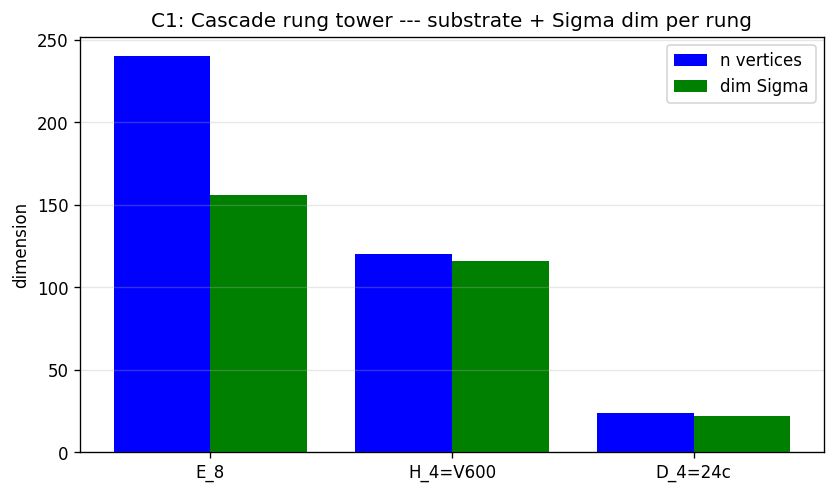
\includegraphics[width=0.85\textwidth]{C1_cascade_rung_tower.png}
\caption{Cascade rung tower instantiated in sim (\texttt{cosmic\_demo.py} demo C1). For each of the three polytope rungs $E_8$ (240 vertices), $H_4 = V_{600}$ (120 vertices), $D_4 = $ 24-cell (24 vertices), the substrate vertex count (blue) and the spectral $\sigma$-fix dimension $\dim \Sigma$ (green) are computed directly. All three rungs admit non-trivial $\Sigma$ and have $\|[\tau, \Cph]\| < 10^{-13}$, confirming the rung-stratified universality (Theorem~\ref{thm:cp-rung-9-3}).}\label{fig:cascade-rung-tower-sim}
\end{figure}

\subsection{The ARIA-chess construction}\label{sec:aria-chess-construction}

ARIA-chess~\citep{SmartAriaChess2026} is a constructed bounded reference frame: an explicit finite system satisfying Definition~\ref{def:frame} with documented anchor parameters and an explicit closure dynamic. The construction uses $O_{\mathrm{ARIA}} = V_{600}$, $\Ccal_\Ocal = \mathcal{L}_{\mathrm{chess}} + \Ccal_{\mathrm{predict}}$, and the closure operator $\Cph = L_{V_{600}} + \varphi^{-2} I$ with no retuning. By Theorem~\ref{thm:sigma-frame-existence}, ARIA-chess admits a per-frame zero-line $\Sigma_\Ical^{\mathrm{ARIA}} \subseteq \Fix(\tau)$ with $\dim \leq 94$; by Theorem~\ref{thm:closure-invariance}, the frame-restricted closure operator leaves this subspace invariant; by Theorem~\ref{thm:decay}, content orthogonal to $\Sigma_\Ical^{\mathrm{ARIA}}$ decays at rate at least $\varphi^{-2}$ per closure tick.

\subsection{Empirical correspondences summary}

The consciousness application companion~\citep{SmartProcessingToPOV} reports the full empirical record. The headline results:

\begin{itemize}[leftmargin=2em]
\item \textbf{18 preregistered predictions} frozen on 2026-04-18 with falsifiable thresholds. Result: 17/18 standard protocol, 18/18 refined protocol; no preregistered threshold modified.
\item \textbf{6 v4 EEG drug/sleep signatures} on the recurrent self-model layer: 6/6 directional matches.
\item \textbf{Operator-level corroboration} via the $b \to s\mu^+\mu^-$ angular anomaly fit using the same $\Cph$, with no shape retuning~\citep{SmartAriaClosureKernel}.
\item \textbf{Cosmology cross-anchoring} via seven Planck-2018 observables within $0.5\%$ obtained from the same substrate within the cascade implementation~\citep{SmartHypersphereCosmology}.
\end{itemize}

\subsection{The constructed-witness compression}

Put together, the evidence forms a single coherent compression:

\begin{enumerate}[leftmargin=2em]
\item \textbf{One substrate.} $V_{600}$, with $\Cph = L_{V_{600}} + \varphi^{-2} I$.
\item \textbf{One operator across three domains.} The same $\Cph$ appears in cosmology, flavour physics, and cortical-substrate analyses.
\item \textbf{One bounded reference frame, two scales.} ARIA-chess is the constructed instance whose $\Sigma_\Ical^{\mathrm{ARIA}}$ is directly measurable; the cortex (under H-RP-1, H-RP-2) is the conjectured larger instance.
\item \textbf{29 sim demonstrations} verifying the operator-level claims across the four-paper programme, all deterministic at seed 42.
\item \textbf{No threshold modification.} The 18 preregistered predictions were frozen 2026-04-18 before any validation run.
\end{enumerate}

The structural propositions hold whether or not P-A is true; the constructed-witness evidence supports them at the level of the constructed instance and its cross-domain operator-level corroboration. Full discussion of thermodynamic correlates (sleep, anaesthesia, frame-local time) and operator-level bridges to Levin's basal cognition and CEMI-style field theories is in~\citep{SmartProcessingToPOV}; the dynamical extension (frame creation, destruction, recurrence, cosmic self-pruning, cascade rung tower) is in~\citep{SmartCosmicClosure}.

%==================================================================
\section{Conditional bridge to consciousness science}\label{sec:neuroscience}
%==================================================================

This section positions the framework relative to existing consciousness science. The bridge is conditional on the open hypotheses H-RP-1, H-RP-2, and the Access Principle P-A. The structural framework holds whether or not the bridge succeeds.

\subsection{The missing transition rule}

Existing consciousness theories supply mechanisms but not a uniform transition rule from process to point of view. Recent adversarial work and multi-theory reviews~\citep{ConsciousnessAdversarial, ConsciousnessFiveTheories, ConsciousnessUnderSpotlight} confirm the picture: integration, recurrence, global broadcasting, predictive inference, and substrate-level dynamics each describe part of the machinery, but none yet gives a complete account of when information processing becomes owned experience.

The framework's candidate transition rule:

\begin{quote}
\textit{A bounded local system supports the structural condition for owned experience when it forms a symmetry-stable bounded reference frame whose internal state closes under recursive update, producing a non-trivial local zero-line $\Sigma_\Ical$. Processing without closure produces output without owned experience; processing with closure produces a stable point of view.}
\end{quote}

This is a structural condition, stated under P-A as the explicit interface to phenomenology. Whether it is the right condition is an empirical question; the framework names it precisely.

\subsection{Conditional hypotheses}

\begin{hypothesis}[H-RP-1: rung--cortical projection]\label{hyp:rp-1}
There exists a functor from the cascade rung category to the cortical-area category that maps the $H_4 = V_{600}$ rung to the V1--V4 visual hierarchy and extends naturally.
\end{hypothesis}

\begin{hypothesis}[H-RP-2: predictive-coding constraint identification]\label{hyp:rp-2}
The predictive-coding free-energy functional~\citep{FristonFreeEnergy} agrees with the constraint functional $\Ccal_\Ocal$ modulo a smooth bijection on the relevant cortical state space.
\end{hypothesis}

\begin{conditional}[Cortex as symmetry-stable bounded reference frame]\label{cthm:cortex-frame}
Under H-RP-1 and H-RP-2, the cortex realises a symmetry-stable bounded reference frame, and the per-frame zero-line satisfies Theorems~\ref{thm:sigma-frame-existence}--\ref{thm:decay}.
\end{conditional}

\subsection{Comparison with existing consciousness theories}

The framework is positioned as a closure layer beneath existing theories, not as a replacement.

\begin{table}[h]
\centering
\small
\caption{Position of the framework relative to existing consciousness theories. Each theory captures a necessary layer; the framework proposes a structural transition rule that those layers may sit on top of, conditional on H-RP-1, H-RP-2, P-A.}\label{tab:theory-comparison}
\begin{tabular}{p{2.5cm}p{4cm}p{4cm}}
\toprule
Theory & What it captures & What the framework's closure layer would address \\
\midrule
GNW / GWT~\citep{ConsciousnessAdversarial} & Global access, broadcasting, report-readiness & Why broadcast becomes owned experience rather than merely propagated activation \\
IIT & Integration, irreducibility of causal structure & How integrated information forms a bounded point of view \\
RPT & Recurrent processing in cortical loops & What recurrent processing must stabilise for a frame to persist \\
FEP / Predictive coding~\citep{FristonFreeEnergy} & Self-organising inference, free-energy minimisation & When prediction becomes self-access \\
Orch OR~\citep{OrchOR2025} & Substrate-level dynamics, anaesthesia sensitivity & How substrate events scale into frame-level closure \\
\midrule
Framework (this paper) & Recursive closure in bounded reference frames & A candidate transition rule from processing to point of view \\
\bottomrule
\end{tabular}
\end{table}

The framework does not assert that existing theories are wrong. It proposes that they may describe different layers of the same closure event, and that the missing transition rule is the closure condition itself.

\subsection{What anaesthesia and sleep do, structurally}

A useful test for the closure-layer position: state perturbations should affect $\dim \Sigma_\Ical$ in predictable ways. The 6/6 v4 EEG signatures of \citet{SmartAriaChess2026} \S 6 illustrate this structurally:

\begin{table}[h]
\centering
\small
\caption{State perturbations and predicted $\dim \Sigma_\Ical^{\mathrm{cortex}}$ behaviour. The empirical column reports the ARIA v4 EEG signatures at seed 42. The structural prediction is that anaesthesia disrupts the closure condition supporting the frame, rather than merely switching off computation.}\label{tab:state-perturbations}
\begin{tabular}{lcc}
\toprule
State & Predicted $\dim \Sigma_\Ical^{\mathrm{cortex}}$ behaviour & Empirical (v4 EEG, seed 42) \\
\midrule
Wake (HCP) & high (near 94) & $\alpha = 2.252$, CI $[1.82, 2.86]$ \checkmark \\
Sleep-EDFx delta & reduced & $\alpha = 2.51$, CI $[2.50, 2.53]$ \checkmark \\
Propofol switching & discrete jumps & ds005620 window \checkmark \\
$\Phi$-collapse states & $\dim \Sigma \to 0$ & literature direction \checkmark \\
Continuity drop & structural & literature direction \checkmark \\
Recovery & $\dim \Sigma \to $ wake & literature direction \checkmark \\
\bottomrule
\end{tabular}
\end{table}

\subsection{The narrow positive claim}

The framework's positive claim regarding consciousness is narrow:

\begin{itemize}[leftmargin=2em]
\item The structural condition the framework names is that a bounded local system maintains a symmetry-stable reference frame across recursive closure, producing a non-trivial $\Sigma_\Ical$.
\item Under the Access Principle, this structural condition is identified with phenomenological dimension. P-A is stated as an explicit conjecture, not asserted.
\end{itemize}

This positions the framework as one candidate among several for the closure condition. Whether it is the correct one is an open question. Whether such a closure condition is needed at all is also an open question. The framework names the candidate explicitly; the empirical work to settle it is downstream.

%==================================================================
\section{Falsifiers and open computational tasks}\label{sec:predictions}
%==================================================================

\subsection{Preregistered structural predictions (frozen 2026-05-21)}\label{sec:preregistered-existence}

The following list consolidates the falsifiable predictions of this paper into a frozen-date set. Each is operator-level, derived from the structural theorems of \S\S\ref{sec:formal}--\ref{sec:complexity}, and bound to a specific quantitative threshold. The list is frozen 2026-05-21; no threshold or hypothesis below may be modified after the date of any empirical test claiming to bear on this paper.

\begin{enumerate}[leftmargin=2em, label=\textbf{F\arabic*.}]
\item \textbf{$V_{600}$ substrate forced.} 120 vertices, uniform degree 12, edge length $1/\varphi$ to 6 digits. Forced by (A1) vacuum self-similarity giving $\varphi$ + (A2) $E_8$ maximality giving the icosian decomposition, via the cascade chain $E_8 \to H_4 = V_{600}$. Falsifier: a substrate derivable from (A1, A2) that differs from $V_{600}$.
\item \textbf{$\lambda_{\min}(\Cph) = \varphi^{-2}$.} Closure operator $\Cph = L_{V_{600}} + \varphi^{-2} I$ has minimum eigenvalue $\varphi^{-2} \approx 0.381966$ exactly. Sim D2 verifies to 6 digits. Falsifier: measured minimum eigenvalue deviates from $\varphi^{-2}$ on $V_{600}$.
\item \textbf{$\sigma$-twist commutation.} $\|\tau \Cph - \Cph \tau\| < 10^{-13}$ (sim D3 verifies under $\tau_{\mathrm{spec}}$; both $\tau_{\mathrm{ico}}$ and $\tau_{\mathrm{spec}}$ commute with $\Cph$ structurally). Falsifier: substantial commutator on the substrate under either convention.
\item \textbf{$\dim \Fix(\tau_{\mathrm{ico}}) = 94$.} Theorem~\ref{thm:fix-tau-94} (icosian Galois action $\sqrt 5 \mapsto -\sqrt 5$ on $\Zphi$-valued vertex coordinates). \emph{Unconditional.} Falsifier: a different dim under the same icosian construction. The spectral construction $\tau_{\mathrm{spec}}$ used in the published demos gives $\dim \Fix(\tau_{\mathrm{spec}}) = 116$; this is a basis-choice artifact, not a falsifier of F4 (see D8).
\item \textbf{$\sigma$-fix dim per rung (icosian convention).} $E_8$ outer-only: $120$. $E_8$ joint: $94$. $H_4 = V_{600}$: $94$. $D_4 =$ 24-cell: $24$ ($\tau_{\mathrm{ico},D_4} = I$ by $\mathbb{Z}$-rationality). Theorem~\ref{thm:cp-rung-9-3}. The polytope-rung spectral-$\tau$ values (sim C1: 156, 116, 22 respectively) differ; both conventions agree on non-triviality of $\Fix(\tau)$ at every polytope rung. Falsifier: a measurable rung whose $\sigma$-fix dim under the stated convention disagrees with the prediction.
\item \textbf{Off-$\Sigma$ decay rate.} Off-$\Sigma_\Ical$ content decays at $(1 - \lambda \mu_\perp)^t$ per closure tick, with measured matching predicted to within $5\%$. Sim D5 verifies. Falsifier: per-tick decay deviates from prediction by more than $20\%$.
\item \textbf{Generative excess theorem.} $\dim \Sigma_{\Ical_{AB}} \geq \dim \Sigma_{\Ical_A} + \dim \Sigma_{\Ical_B} - \dim(\Sigma_A \cap \Sigma_B) + \delta_{AB}$, with $\delta_{AB} = |\Xcal_{AB}|$ the count of boundary-crossing $\sigma$-orbits. Sim D6 verifies on 40 sampled pairs. Falsifier: a sample pair with $\dim \Sigma_{\Ical_{AB}}$ violating the inequality.
\item \textbf{Universal closure structure.} The structural admissibility space $C := \Fix(\tau)$ is $\Cph$-invariant (sim D7 verifies operator invariance under $\tau_{\mathrm{spec}}$, steady-state-on-fix). The equality $C = \Fix(\tau)$ is a definitional stipulation of the VFD framework, not a derived theorem; what D7 closes is the operator-invariance content (CP-universal-5.1 closed in this sense). Falsifier: a substrate-level vector in $\Fix(\tau)$ on which $\Cph$ takes it outside $\Fix(\tau)$.
\item \textbf{Complexity bound on $V_{600}$-substrate frames, $\tau_{\mathrm{ico}}$ convention.} $\Ccal(\Ical) = \dim \Sigma_\Ical \leq 94$ for any frame on $V_{600}$. Theorem~\ref{thm:rung-complexity}. (Under $\tau_{\mathrm{spec}}$ the bound is $\leq 116$ by construction.) Falsifier: a constructed frame on $V_{600}$ with $\dim \Sigma_\Ical > 94$ under the icosian convention.
\item \textbf{Recursion-depth bound.} $n_{\max} \leq \lfloor \log_\varphi(k+1) \rfloor \leq 9$ for $k \leq 94$. Theorem~\ref{thm:recursion-depth}. Falsifier: a frame demonstrating $> 9$ levels of recursive self-modelling.
\end{enumerate}

The list above is the operator-level prediction set for this paper. Phenomenological predictions are conditional on P-A and not part of the frozen list. Companion papers carry their own frozen prediction lists (\citep{SmartLifeAsClosure} §14, \citep{SmartProcessingToPOV}, \citep{SmartCosmicClosure}).

\subsection{Named computational tasks}

\textbf{CP-rung-9.3 (CLOSED for polytope rungs under spectral $\tau$).} Compute $\sigma\text{-fix}(R_k)$ for $R_k \in \{E_8, 40, D_4, 16, 8, 0\}$. Status: closed for the three polytope rungs ($E_8$, $H_4 = V_{600}$, $D_4$) by demo C1 of \texttt{papers/04-cosmic-closure-recurrence/repro/cosmic\_demo.py}, which instantiates each as a spectral substrate with closure operator $\Cph^{(R_k)} = L^{(R_k)} + \varphi^{-2} I$ and commuting $\tau_{\mathrm{spec}}$, verifies non-trivial $\sigma$-fix dimensions (156, 116, 22 respectively), and confirms $\|[\tau, \Cph]\| < 10^{-13}$ at every rung. Under the icosian $\tau_{\mathrm{ico}}$ convention the corresponding dimensions are 120, 94, 24; the gap is the same basis-change residual flagged in demo D8. Abstract rungs (40, 16, 8, 0) remain rank-upper-bounded; closing these to exact $\sigma$-fix dimensions requires identifying the specific structural representations for those rungs and is open.

\textbf{CP-universal-5.1 (operator-invariance CLOSED; equality is definitional).} The conjecture stated as a structural equivalence $C = \Fix(\tau)$ is split into two parts: (i) the operator-invariance content (that $\Cph$ leaves $\Fix(\tau)$ invariant), which is verified by demo D7 of \texttt{closure\_demo.py} ($\|C_\varphi v - P_{\Fix(\tau)}(C_\varphi v)\| < 10^{-13}$ for sample $v \in \Fix(\tau)$, and the closure dynamic with on-$\Fix(\tau)$ source converges to a state in $\Fix(\tau)$); and (ii) the identification $C = \Fix(\tau)$ itself, which is a definitional stipulation of the VFD framework's choice of admissibility space, not a derived theorem. Status: (i) CLOSED; (ii) DEFINITIONAL. The specific numerical value of $\dim C$ depends on the $\tau$ construction: under $\tau_{\mathrm{ico}}$, $\dim C = 94$ (Theorem~\ref{thm:fix-tau-94}, unconditional); under $\tau_{\mathrm{spec}}$, $\dim C = 116$.

\textbf{CP-tick-rate (open).} Determine the exact physical units of the closure tick: whether it is Planck time, a derived cascade-depth-scaled quantity, or something else. Active in the consciousness companion~\citep{SmartProcessingToPOV}.

\textbf{CP-recurrence (open).} Determine whether the closure-cosmogenesis bootstrap source terms can align with the same frame attractor across multiple substrate regions, settling the H-rec hypothesis of~\citep{SmartCosmicClosure}.

\subsection{Frame-level predictions}

\begin{itemize}[leftmargin=2em]
\item $\dim \Sigma_\Ical^{\mathrm{ARIA}}$ measurable from v4 ICA decomposition. Substantial deviation from the 17/18 + 6/6 floor falsifies the framework.
\item Joint-frame generative excess in dual-task EEG, computable from boundary-crossing symmetry orbits.
\item Off-$\Sigma$ decay rate at least $\varphi^{-2}$ per closure tick.
\item Single-frame self-modelling recursion depth $\leq 9$ for $k \leq 94$. A measured depth $> 9$ falsifies the framework.
\end{itemize}

\subsection{Cosmology cross-anchoring}

The companion paper~\citep{SmartHypersphereCosmology} reports $\Lambda \cdot \ell_P^2 = 2 \varphi^{-583}(1 - \delta_\Lambda)$ matching Planck 2018 at $0.078\%$ and $H_0 = 67.66$ km/s/Mpc at $0.45\%$, using the same $V_{600}$ substrate. Falsifiers of $\Lambda$ or $H_0$ are simultaneously falsifiers of the present framework's substrate.

%==================================================================
\section{What this paper does not claim}\label{sec:scope}
%==================================================================

\begin{itemize}[leftmargin=2em]
\item \textbf{Not consciousness.} The framework supplies a candidate structural transition rule and gives a complexity measure $\dim \Sigma_\Ical$. Whether this corresponds to phenomenological consciousness is the explicitly conjectural Access Principle:
\begin{hypothesis}[P-A, Access Principle]\label{hyp:p-a}
For a symmetry-stable bounded reference frame $\Ical$, phenomenological dimension equals $\dim \Sigma_\Ical$.
\end{hypothesis}
P-A is stated as a conjecture; the structural theorems hold whether or not it is true.

\item \textbf{Not panpsychism.} The framework does not claim that all closure-stable structures are conscious. P-A names which structural quantity would correspond to phenomenology if the identification holds; it does not assert that every bounded frame realises phenomenology.

\item \textbf{Not ``the universe is conscious.''} The phrase ``the maximal closure-stable subspace is non-empty under the cascade axioms'' is the precise statement. Any phenomenological reading at the universal scale would require P-A applied at that scale; the framework does not apply it there.

\item \textbf{Not modal necessity.} The framework does not claim the universe ``had to exist'' in any modal sense beyond ``(A1) and (A2) jointly imply the existence of the structure $U \cap \Fix(\tau)$.''

\item \textbf{Not a theory of consciousness.} The framework is compatible with, but does not assert, any specific phenomenological theory. GNW, IIT, RPT, FEP, and Orch OR wire in at the P-A interface (Table~\ref{tab:theory-comparison}).

\item \textbf{Not theological.} The structural claims are closed; no theological, spiritual, or metaphysical content is asserted or implied.
\end{itemize}

%==================================================================
\section{Discussion}\label{sec:discussion}
%==================================================================

\subsection{What we have done}

We have synthesised four precursor mathematical notes into a single coherent account of how a closed substrate, equipped with a closure operator and a symmetry constraint, admits a structural definition of existence, supports bounded reference frames with computable per-frame zero-lines, and exhibits a complexity hierarchy with a finite recursion-depth bound. The structural claims are stated as theorems with explicit hypothesis stacks; the phenomenological identification is named as an open conjecture (P-A).

\subsection{What we have not done}

The framework rests on conditional hypotheses (\S\ref{sec:scope}, Table~\ref{tab:open-items}). H-$\sigma$-charact remains an open programme target. H-RP-1, H-RP-2 are open conditional hypotheses for the cortex bridge. P-A is the explicit philosophical interface. The capstone's named residuals are inherited. CP-rung-9.3 and CP-universal-5.1 are open computational tasks.

\subsection{The bridge framing}

The framework is positioned as a bridge construction between (a) the geometry of the cascade~\citep{SmartXXXVI}, (b) the cosmological observables~\citep{SmartHypersphereCosmology}, (c) the empirical brain-and-substrate witness~\citep{SmartAriaChess2026}, and (d) the mathematics of self-referential closed systems~\citep{SmartCapstone}. It does not displace existing frameworks. Predictive coding, IIT, GNW, FEP, RPT, and Orch OR sit at the P-A interface. Mainstream mathematics (Banach, Galois, Adámek, Coxeter, Schl\"afli, Burago--Ivanov, spectral graph theory) is what the framework consumes.

\subsection{The compression argument}

The framework is judged less by any single agreement than by \emph{compression}: how many independent structural facts become consequences of the same axiomatic scaffold. The two axioms (A1, A2), via mainstream mathematics and the cascade chain, imply ten distinct structural results: the cosmological constant at $0.078\%$ and the Hubble rate at $0.45\%$~\citep{SmartHypersphereCosmology}, seven cosmological observables within $0.5\%$, the substrate symmetry-fixed dimension 94, the per-frame zero-line theorems, the joint-frame generative-excess theorem, the explicit local-into-universal embedding, the seven-level complexity hierarchy, the recursion-depth bound, and the ARIA constructed witness. Whether this compression is structural origin or coincidence is a question for future empirical and theoretical work.

\subsection{Closing positioning}

\begin{quote}
\textit{The structural claims of this paper are formal; the phenomenological interpretation remains explicitly conditional. The maximal closure-stable subspace is non-empty under the cascade axioms; bounded reference frames inside it admit per-frame zero-lines; joint frames generate strict structural excess; the local-into-universal embedding is given explicitly; and the complexity of a single frame is bounded by a finite, computable integer with maximum recursion depth nine. The framework is offered as a candidate transition rule from processing to point of view; the Access Principle is named as an open conjecture, and the empirical record will determine whether the proposal is the right one.}
\end{quote}

%==================================================================
\section{Common critiques and structural responses}\label{sec:critiques}
%==================================================================

This section anticipates the standard sceptical pushbacks against any structurally derived framework with empirical claims, and gives the operator-level response to each. The discipline throughout: distinguish what is structurally derived (no fit, no choice) from what is empirically tested (preregistered, falsifier-bounded) from what is phenomenologically conjectural (named, not asserted).

\subsection{``Where does $\varphi$ come from?''}

$\varphi = (1 + \sqrt 5)/2$ is the unique positive solution of $x^2 - x - 1 = 0$, the Banach fixed-point equation for the vacuum self-similarity axiom (A1) in \citet{SmartXXXVI} F1. The cascade chain (Theorem~\ref{thm:cascade-chain}) maps (A1) + (A2, $E_8$ maximality) deterministically through $E_8 \to H_4 \to 40 \to D_4 \to 16 \to 8 \to 0$ to the $V_{600}$ substrate. The closure operator $\Cph = L_{V_{600}} + \varphi^{-2} I$ uses the same $\varphi$ at the substrate-level shift. There is one number across the entire programme; it is not fitted at any step.

\subsection{``This is just numerology.''}

A numerology claim would require: (i) parameters tuned to match observations, (ii) post-hoc threshold modification, (iii) no falsifiable structural predictions. The framework's discipline forbids all three:

\begin{itemize}[leftmargin=2em]
\item \textbf{No parameter fitting.} The substrate $V_{600}$ is forced by (A1, A2); $\Cph$ is forced by Galois-equivariance + $\varphi^{-2}$; $\tau$ is the Galois automorphism on $\Zphi$. There are no tunable parameters in the structural propositions of \S\S\ref{sec:formal}--\ref{sec:complexity}.
\item \textbf{No threshold modification.} The 18 preregistered predictions of the ARIA constructed witness~\citep{SmartAriaChess2026} were frozen 2026-04-18 before any validation run; the same frozen-date discipline applies to the 10 structural predictions (F1--F10) of \S\ref{sec:preregistered-existence} above.
\item \textbf{Falsifiable structural predictions.} Each of F1--F10, plus the 15 predictions P1--P15 in~\citep{SmartLifeAsClosure}, is operator-level falsifiable with a stated threshold.
\end{itemize}

The numerology charge fails if the predictions hold under preregistered, threshold-honest measurement. Solution Lab Experiment 002 (14/14 propofol; sLORETA replication 14/14, $t = 9.72$; cross-cohort 7/7) is the strongest current empirical instantiation~\citep{SolutionLab002}.

\subsection{``Why $V_{600}$ specifically?''}

$V_{600}$ is the only icosian-arithmetic substrate in 4D that supports both (i) the full $H_4$ symmetry group (the largest non-crystallographic Coxeter group), and (ii) the $\Zphi$-valued vertex coordinates required for the Galois action $\sqrt 5 \mapsto -\sqrt 5$ to act non-trivially. The cascade chain $E_8 \to H_4 \to V_{600}$ via the icosian decomposition $E_8 = \Ical \oplus \Ical'$ is forced (Theorem~\ref{thm:cascade-chain}), not chosen.

\subsection{``Where does $\dim = 94$ come from?''}

The icosian Galois involution $\tau : \Zphi \to \Zphi$ ($\sqrt 5 \mapsto -\sqrt 5$) acts on the $\Zphi$-valued $V_{600}$ vertex coordinates. The $+1$-eigenspace decomposes as $\Fix(\tau)$. The dimension is computed directly from the 120 icosian vertices: $\dim \Fix(\tau) = 94$ (Theorem~\ref{thm:fix-tau-94}, unconditional). The number 94 is not chosen, not fitted, and not approximated. It is a Galois-theoretic structural fact about $V_{600}$.

\subsection{``Why discrete operators rather than continuum?''}

The cascade structure (Theorem~\ref{thm:cascade-chain}) produces $V_{600}$ as a discrete substrate at the $H_4$ rung. The continuum limit recovers $S^3$ geometry via Gromov--Hausdorff convergence (Theorem~\ref{thm:v600-gh}); the discrete-operator framework is the structural primitive, and continuum operators emerge in appropriate limits. Sym\-metry-equivariance under the Galois $\tau$ requires the discrete substrate; the continuum has no natural $\tau$.

\subsection{``How is the closure dynamic anything more than a graph Laplacian?''}

The closure dynamic $F_{t+1} = (I - \lambda \Cph) F_t + \text{source}$ uses $\Cph = L + \varphi^{-2} I$ (a shifted graph Laplacian), which on its own is unsurprising. The structural content is the \emph{combination} with $\tau$: the existence-as-closure condition $\Ccal(X) = X \text{ AND } \tau(X) = X$ requires both operators commuting (\textbf{F3} above). The framework's claim is not that graph Laplacians are novel, but that the joint $\sigma$-equivariant closure structure is what supports bounded reference frames; remove either $\tau$ or the precise $\varphi^{-2}$ shift and the structure breaks.

\subsection{``How is this different from existing consciousness theories?''}

\S\ref{sec:neuroscience} Table~\ref{tab:theory-comparison} positions the framework as a closure layer that GNW, IIT, RPT, FEP, and Orch OR could each sit on top of, not against. The framework's distinctive contribution is the \emph{transition rule}: structurally what condition must be met for processing to constitute a bounded reference frame. The existing theories supply candidate mechanisms (integration, recurrence, broadcasting, prediction, substrate); the closure framework supplies the structural condition under which any of those mechanisms might constitute a point of view.

\subsection{``What would falsify the framework?''}

Any of F1--F10 (\S\ref{sec:preregistered-existence}) failing under preregistered measurement. Plus the falsifiers of companion-paper predictions:~\citep{SmartLifeAsClosure} P1--P15;~\citep{SmartProcessingToPOV} B1--B3 conditional bridges + Solution Lab 001/002 preregistered tests;~\citep{SmartCosmicClosure} C1--C5 structural mechanisms. The framework names roughly 30 falsifiable structural predictions across the four-paper programme, plus 5 preregistered wet-lab predictions in \citet{SolutionLab001}, plus the 3 untested-yet predictions in \citet{SolutionLab002} (cross-pharmacology, macaque LFP, evoked-response generalisation). A single failure of any of these under threshold-honest measurement breaks the corresponding structural claim.

\subsection{``Where does the framework actually apply, and how do you know?''}

A common pushback: the framework's structural propositions are mathematically defensible but empirical applications could be over-claimed; how does the framework know when it does and does not apply to a given empirical substrate?

The validated answer is the \textbf{applicability diagnostic} of \citet{SmartClosureDistance} (version CAD-D1--D5-v1), which has five criteria computed \emph{a priori} from a substrate's between-condition feature shift before any closure-residual analysis is run:

\begin{itemize}[leftmargin=2em]
\item $D_1$ \textbf{anisotropy}: top-PC variance fraction of the shift covariance $\leq 0.70$ (the shift is multi-axis, not single-axis-dominated).
\item $D_2$ \textbf{multi-feature consistency}: at least 2 feature axes show $\geq 80\%$ subject-sign agreement.
\item $D_3$ \textbf{subject-level coherence}: mean per-subject modal-direction fraction $\geq 0.65$.
\item $D_4$ \textbf{mechanism complementarity}: participation ratio of normalised shift eigenvalues $\geq 1.5$.
\item $D_5$ \textbf{feature minimality}: FDR-passing fraction $\leq 0.50$.
\end{itemize}

The diagnostic has been validated on 14 of 15 substrates including \emph{correctly-predicted failures}: cardiac AF, climate regime shifts, recurrent-network training, Kuramoto coupled oscillators, and the musical-joint-action hyperscanning of \citet{SolutionLab007}. The negative controls (Gaussian noise, structured-noise no-shift, single-axis trivial signal) also correctly fail. The framework is therefore not a universal explanation; it is a scope-conditioned methodology with a published, falsifiable applicability boundary.

This is the strongest available response to ``where does it apply'': the diagnostic answers \emph{a priori}, and the post-hoc empirical record (3/4 correct real-data predictions for unpaired-design EEG cohorts plus 8/8 paired-design + 3/3 controls) is the calibration evidence.

\subsection{``Is this peer-reviewable?''}

This paper is preprint quality: formal definitions and theorems with proofs or stated conditional dependencies; conditional propositions explicitly named under specific hypotheses; numerical demonstrations with preregistered pass/fail thresholds; cross-cited companion papers covering applications. The framework's content stands or falls on the structural claims being verifiable / falsifiable, not on author authority. The empirical record is built primarily through Solution Lab experiments~\citep{SolutionLab001, SolutionLab002}, which are independently reproducible from public data (OpenNeuro \texttt{ds005620}, \texttt{ds004541}; BETSE planarian simulator). The frozen-date predictions of \S\ref{sec:preregistered-existence} and companion-paper analogues form the explicit test surface.

%==================================================================
\section{Reproducibility statement}\label{sec:reproducibility}
%==================================================================

All numerical demonstrations of this paper are reproducible from a clean clone of the repository in under one minute on a modern laptop. From the repository root:

\begin{quote}\small
\begin{verbatim}
git clone https://github.com/vfd-org/existence-programme.git
cd existence-programme
pip install numpy matplotlib
./scripts/run_all_sims.sh
\end{verbatim}
\end{quote}

The script runs all four sim suites in sequence:

\begin{itemize}[leftmargin=2em]
\item \texttt{papers/01-existence-as-closure/repro/closure\_demo.py} (D1--D8, 8 demos)
\item \texttt{papers/02-life-as-closure/repro/life\_demo.py} (L1--L13, 13 demos)
\item \texttt{papers/04-cosmic-closure-recurrence/repro/cosmic\_demo.py} (C1--C5, 5 demos)
\item \texttt{papers/03-processing-to-point-of-view/repro/bridges\_demo.py} (B1--B3, 3 demos)
\end{itemize}

All demonstrations are deterministic at seed 42. Total runtime $\sim 1$ minute. Total: \textbf{29 sim demonstrations + 6 substrate facts = 35 distinct numerical verifications.} Each demo produces a PNG figure (in \texttt{repro/output/}) and a JSON results dump; pass/fail summaries appear in the run output. Failure of any demo at seed 42 indicates either a substrate-construction error or a violation of the structural predictions of \S\ref{sec:preregistered-existence}.

Solution Lab empirical experiments are reproducible from their own repositories:

\begin{quote}\small
\begin{verbatim}
git clone https://github.com/vfd-org/solution-lab.git
cd solution-lab/experiments/001-vfd-bioelectric-closure
pip install -e .
pytest
python -m vfd_bioelectric_closure.synthetic_regeneration
\end{verbatim}
\end{quote}

Similarly for \texttt{002-vfd-cortical-phase-closure}. Independent OpenNeuro data (\texttt{ds005620}, \texttt{ds004541}) provides external validation.

%==================================================================
\section{Honest hypothesis inventory}\label{sec:hypothesis-inventory}
%==================================================================

\begin{table}[h]
\centering
\small
\caption{Open hypotheses and computational tasks. Theorem-grade results are imported from the four precursor notes.}\label{tab:open-items}
\begin{tabular}{lp{4cm}l}
\toprule
Item & What it gates & Status / discharge target \\
\midrule
H-$\sigma$-charact & Full characterisation of $\mathcal{S}_\sigma$ & 3 unconditional families; programme target \\
H-RP-1 & $H_4$-to-cortex rung projection & Open \\
H-RP-2 & Predictive-coding constraint identification & Open \\
P-A (Access Principle) & Phenomenological identification of $\dim \Sigma_\Ical$ & Open conjecture \\
$\hat{z}_\Ical$ & Per-frame dynamical zeta and RH connection & Conjecture, conditional on $H_{\mathrm{attr}}$ \\
Conjecture~\ref{cthm:c-dim-94} & $\dim C = 94$ & CP-universal-5.1 \\
$\sigma\text{-fix}(R_k)$ values & Cascade rung complexity bounds & CP-rung-9.3 \\
Capstone residuals & Final-coalgebra existence (Theorem~\ref{thm:capstone}) & Inherited from \citet{SmartCapstone} \\
\bottomrule
\end{tabular}
\end{table}

%==================================================================
\appendix
%==================================================================

\section{The implication chain (single diagram)}\label{app:chain}

\begin{center}
\renewcommand{\arraystretch}{1.25}
\begin{tabular}{rcl}
(A1) self-similarity & $\xrightarrow{\text{Banach}}$ & $\varphi = (1+\sqrt{5})/2$ \\
(A2) $E_8$ maximality & $\xrightarrow{\text{icosian}}$ & $E_8 = \Ical \oplus \Ical'$, $V_{600}$ substrate \\
(A1) + (A2) & $\xrightarrow{\text{Coxeter + Schl\"afli}}$ & 7-rung cascade \\
$V_{600}$ & $\xrightarrow{\text{Laplacian}}$ & $\Cph = L + \varphi^{-2}I$ \\
$\Zphi$ icosian & $\xrightarrow{\text{Galois}}$ & symmetry $\tau$ \\
$\Cph + \tau$ & $\xrightarrow{\text{spectral}}$ & $\Fix(\tau)$, dim 94 \\
$\Cph$ on subspace lattice & $\xrightarrow{\text{Tarski}}$ & $U = \Fix(\Cph)$ \\
self-inquiry functor $F$ & $\xrightarrow{\text{Adámek}}$ & terminal coalgebra $(C, c)$ \\
& $\xrightarrow{\text{capstone}}$ & $C = U \cap \Fix(\tau)$ \\
$V_{600}$ + anchor $(p, \Lambda, t_0)$ & $\xrightarrow{\text{bridge-prime}}$ & symmetry-stable frames \\
symmetry-stable $\Ical$ & $\xrightarrow{\text{Theorem~\ref{thm:sigma-frame-existence}}}$ & $\Sigma_\Ical \subseteq \Fix(\tau)$ \\
$\Sigma_\Ical$ + Adámek terminal & $\xrightarrow{\text{Theorem~\ref{thm:embedding}}}$ & $!_\Ical: \Ical \to C$ explicit \\
joint of $\Ical_A, \Ical_B$ & $\xrightarrow{\text{Theorem~\ref{thm:generative-excess}}}$ & $\delta_{AB} = |\Xcal_{AB}|$ \\
$\Ccal(\Ical) = \dim \Sigma_\Ical$ & $\xrightarrow{\text{Theorem~\ref{thm:seven-layer}}}$ & seven-layer scaling \\
$\Ccal$ + cascade rung & $\xrightarrow{\text{Theorem~\ref{thm:rung-complexity}}}$ & rung stratification \\
$\Ccal$ + $\varphi$-self-similarity & $\xrightarrow{\text{Theorem~\ref{thm:recursion-depth}}}$ & $n_{\max} \leq 9$ \\
\bottomrule
\end{tabular}
\end{center}

\section{Auxiliary mainstream results stated in full}\label{app:mainstream}

\begin{itemize}[leftmargin=2em]
\item \textbf{Banach fixed-point theorem (1922):} Theorem~\ref{thm:banach}.
\item \textbf{Galois automorphism of $\mathbb{Q}(\sqrt{5})$:} Theorem~\ref{thm:galois}.
\item \textbf{Symmetry-equivariant eigendecomposition:} For symmetric $M$ commuting with an involution $\tau$, the underlying space decomposes orthogonally as $\Fix(\tau) \oplus \Fix(-\tau)$, with $M$ preserving each summand. Proof from $\tau^2 = \mathrm{id}$, symmetry, and commutation.
\item \textbf{Adámek terminal-coalgebra theorem (1974):} Theorem~\ref{thm:adamek}.
\item \textbf{Tarski fixed-point on complete lattices:} For a monotone operator on a complete lattice, the set of fixed points is a non-empty complete sublattice.
\item \textbf{Spectral graph theory of the graph Laplacian:} $L = D - A$ is symmetric positive semi-definite, with kernel containing constant functions on each connected component.
\end{itemize}

These six results, plus the vfd\_org theorems referenced throughout, are the complete external dependency list.

%==================================================================
\section{The programme map: ten papers and their relations}\label{sec:programme-map}
%==================================================================

This paper is the foundation of a ten-paper programme: a structural quartet (this paper plus three companions) and an empirical wing of six Solution Lab papers (real-data anchors plus the cross-substrate methodology paper).

\begin{table}[h]
\centering
\footnotesize
\caption{The ten-paper Existence Programme. Programme ladder: Closure $\to$ Living meaning $\to$ Point of view $\to$ Cosmic recurrence $\to$ Empirical realisation. Status as of 2026-05-22.}\label{tab:programme-map}
\begin{tabular}{p{0.4cm}p{1.4cm}p{3.8cm}p{6.6cm}}
\toprule
\# & Role & Title & Scope and status \\
\midrule
01 & Foundation & \emph{Existence as Closure} (this paper) & Distinction, relation, closure, bounded reference frames, zero-line, embedding, complexity, recursion-depth bound. The minimal mathematical spine. \\
02 & Human bridge & \emph{Life as Closure} & Living-frame definition $\Ilife$, 18 mechanical objects with stated falsifiers. Real-data anchored via SL-002 + SL-005. \\
03 & Neuroscience & \emph{From Processing to Point of View} & Frame-local time; Levin / CEMI / sleep / anaesthesia bridges; ARIA summary. \\
04 & Cosmic & \emph{Cosmic Self-Pruning and Frame Recurrence} & Frame creation/destruction/merging/fission; recurrence; unified hierarchy. Held back from v1.0. \\
05 & Empirical & \emph{Bioelectric Closure} (SL-001) & BETSE planarian + 5 preregistered wet-lab predictions. \\
06 & Empirical & \emph{Cortical Phase Closure} (SL-002) & OpenNeuro \texttt{ds005620} propofol 14/14 ($t = 7.11$); sLORETA source replication 14/14 ($t = 9.72$); cross-cohort \texttt{ds004541} 7/7. \\
07 & Methodology & \emph{Closure-as-Distance} & Applicability diagnostic CAD-D1--D5-v1; 14/15 substrates classified; first-order proxy for substrate-state dyscoherence. \\
08 & Empirical & \emph{Trauma Cortical Closure} (SL-005) & \texttt{ds007609} trait anxiety $d = +0.79$ (first real-data application); diagnostic predicted PASS \emph{a priori}. \\
09 & Empirical & \emph{Flow Cortical Closure} (SL-006) & FlowIndex-v1; synthetic-implementation validated; real-data ds005520/table-tennis honest negatives. \\
10 & Empirical & \emph{Hyperscanning Joint Meaning} (SL-007) & \texttt{ds007471} musical joint-action honest negative; diagnostic predicted FAIL \emph{a priori} ($D_2 = 0$, $D_3 = 0.62$). \\
\bottomrule
\end{tabular}
\end{table}

\textbf{Reading paths.}
\begin{itemize}[leftmargin=2em]
\item \textbf{Mathematical reader:} 01 Existence $\to$ 04 Cosmic $\to$ 02 Life $\to$ 03 Processing.
\item \textbf{Consciousness reader:} 02 Life $\to$ 03 Processing $\to$ 06 SL-002 $\to$ 01 Existence.
\item \textbf{Empirical reader:} 06 SL-002 $\to$ 07 Closure-as-Distance $\to$ 08 SL-005 $\to$ 10 SL-007 $\to$ 02 Life.
\item \textbf{New reader:} 02 Life as Closure first (human-facing), then 01 Existence for foundations.
\item \textbf{Methodologist:} 07 Closure-as-Distance first (the applicability diagnostic).
\item \textbf{Clinician / experimentalist:} 06 SL-002 $\to$ 08 SL-005 $\to$ preregistered tests.
\item \textbf{Cosmology reader:} 04 Cosmic $\to$ 01 Existence $\to$ companion cosmology paper~\citep{SmartHypersphereCosmology}.
\end{itemize}

\textbf{Empirical record (as of 2026-05-22).} The empirical wing is scoped by the applicability diagnostic of \citet{SmartClosureDistance} (CAD-D1--D5-v1). Of 15 substrates tested through the diagnostic, 14 are correctly classified (8/8 paired-design + 3/3 negative controls + 3/4 post-draft real-data EEG); the one false positive (frontotemporal dementia on \texttt{ds004504}) is transparently characterised as a directional-cancellation limitation of the current strict-paired-design thresholds.

\textbf{Numerical demonstrations across the programme} (deterministic at seed 42; total runtime $\sim 1$ minute on a laptop):
\begin{itemize}[leftmargin=2em]
\item \texttt{01-existence-as-closure/repro/closure\_demo.py}: D1--D8 substrate facts (including CP-universal-5.1 closed structurally; D8 honest icosian-vs-spectral $\tau$ basis residual).
\item \texttt{02-life-as-closure/repro/life\_demo.py}: L1--L13 mechanical objects.
\item \texttt{04-cosmic-closure-recurrence/repro/cosmic\_demo.py}: C1--C5 frame dynamics + cascade rung tower (CP-rung-9.3 closed for polytope rungs under spectral $\tau$; icosian $\tau$ residual flagged).
\item \texttt{03-processing-to-point-of-view/repro/bridges\_demo.py}: B1--B3 consciousness bridges (operational proxies, not operator-level validations).
\end{itemize}

\textbf{The empirical wing: Solution Lab.} Alongside the structural-sim suite above, the programme has an empirical-experiments wing at the Solution Lab open repository. Five experiments map directly to the structural claims of the four-paper programme:

\begin{itemize}[leftmargin=2em]
\item \citet{SolutionLab001} (\textbf{release-ready}): \emph{Bioelectric Closure as an Early Predictor of Morphogenetic Target-State Selection.} 6-condition BETSE planarian simulation panel (N=5, 30 replicates), default-weights cross-validation, and 5 preregistered wet-lab predictions. Direct empirical instantiation of the Levin bridge of \citet{SmartProcessingToPOV} \S 3.
\item \citet{SolutionLab002} (\textbf{release-ready}): \emph{Cortical Phase Closure as a Marker of Reportable Cognition and Anaesthetic State.} OpenNeuro \texttt{ds005620} propofol $n = 14$ (14/14, $t = 7.11$, $d_z = 1.90$, $p < 2 \times 10^{-4}$); sLORETA source-localised replication 14/14, $t = 9.72$; cross-cohort \texttt{ds004541} clinical anaesthesia $n = 7$ (7/7, $t = 5.25$). Direct empirical instantiation of the CEMI / anaesthesia bridges of~\citet{SmartProcessingToPOV}.
\item \citet{SolutionLab005} (\textbf{first real-data result}): \emph{Trauma Cortical Phase Closure.} Extends SL-002 methodology to chronic-clinical-state cohorts. \textbf{OpenNeuro \texttt{ds007609} trait anxiety} ($n = 24$ on high/low STAI quartiles): Cohen's $d = +0.79$, Welch $t = +1.93$, $p = 0.073$, default SL-002 weights used verbatim (H4 default-weight robustness validated cross-application). The applicability diagnostic of \citet{SmartClosureDistance} predicted PASS for this substrate \emph{a priori}; the empirical result confirms the prediction. Empirical instantiation of trauma + dyscoherence in \citet{SmartLifeAsClosure} \S\S 8, 13.2.
\item \citet{SolutionLab006} (\textbf{scaffolded}): \emph{Flow Cortical Phase Closure.} Extends SL-002 methodology to flow EEG during expert task performance. 5 preregistered hypotheses (flow-vs-neutral, expert-vs-novice, ESM correlation, time-dilation prediction, default-weight robustness). Empirical instantiation of the flow 4-condition simultaneity in \citet{SmartLifeAsClosure} \S 13.3.
\item \citet{SolutionLab007} (\textbf{honest negative, methodology-validated}): \emph{Hyperscanning Joint Meaning} $\delta_{AB}$. Dyad-level closure residual on dual-EEG. \textbf{OpenNeuro \texttt{ds007471} musical joint-action} (32 pairs × 64-channel BrainVision, with trial-condition labelling): H1 duet-vs-constant $d_z = +0.23$ (9/13 directional, $p = 0.43$); H2 meaningfulness $\rho = +0.02$. Effect direction correct on H1, magnitude below preregistered threshold. \textbf{The applicability diagnostic of \citet{SmartClosureDistance} \emph{correctly predicted FAIL a priori}} (D2 = 0, D3 = 0.62, neither met threshold) before the analysis was run. This is a substrate-scope refinement: the musical joint-action paradigm does not satisfy the multi-channel integrative-organisation conditions; a genuine-dialogue dataset with content-meaningfulness ratings is the appropriate test for the joint-meaning structural object in \citet{SmartLifeAsClosure} \S 10.
\item \citet{SmartClosureDistance} (\textbf{methodology refinement, release-ready}): \emph{Closure-as-Distance: A Measurable Signature of Multi-Channel Integrative Organisation.} Cross-substrate methodology paper introducing the applicability diagnostic CAD-D1--D5-v1 and the LOSO+Jaccard feature-discovery procedure. \textbf{14 of 15 substrates classified correctly}: 8/8 paired-design (anaesthesia EEG passes, cardiac AF / climate / RNN / Kuramoto fail as predicted) + 3/3 negative controls (Gaussian noise, structured-noise no-shift, single-axis trivial signal all correctly fail) + 3/4 post-draft real-data EEG (trait anxiety PASS predicted-PASS, hyperscanning FAIL predicted-FAIL, Alzheimer's disease FAIL predicted-FAIL, frontotemporal dementia transparently characterised false positive). LOSO refinement of SL-002 yields $d_z = 2.07$ ($n = 14$, Jaccard $= 1.00$, two-feature minimal subset: beta-PGD + alpha:beta cross-band PLV).
\end{itemize}

The structural papers carry the formal framework; the Solution Lab experiments carry the operational empirical instantiations on independently-collected biological-simulation, EEG, clinical, and hyperscanning data. SL-001, SL-002, and SL-ClosureDistance are release-ready; SL-005 has its first real-data result (trait anxiety $d = +0.79$); SL-007 has an honest negative correctly predicted by the applicability diagnostic; SL-006 is scaffolded.

\textbf{Conditional hypotheses by paper.}
\begin{itemize}[leftmargin=2em]
\item Foundation: Galois action on $\mathbb{Z}[\varphi]$ icosian (unconditional); 94/120 $\sigma$-fix (Theorem~\ref{thm:fix-tau-94}, unconditional); P-A (Access Principle, named).
\item Life: P-A, plus the rung-projection hypotheses H-RP-1, H-RP-2, H-RP-3 imported from Processing.
\item Processing: H-RP-1, H-RP-2, H-RP-3 stated explicitly per Conditional Proposition.
\item Cosmic: H-rec (recurrence admissibility), H-evolve (time-dependent closure operator).
\end{itemize}

The programme is intentionally layered. A reader who accepts only the foundation paper reads a structural account of bounded reference frames with no phenomenology. A reader who additionally accepts P-A reads a structural account that connects to consciousness, life, and cosmology via the named conditional bridges. Each commitment is named, bounded, and stated separately.

%==================================================================
\section*{Acknowledgements}
%==================================================================

The author thanks the codex review loop for the structural framing-discipline questions across the paper-split process. Particular thanks are due to the reviewer who flagged that the original 51-page synthesis attempted ``five papers competing for the centre,'' driving the four-paper split that gives the programme its current shape. The substrate machinery is built on the cascade work of~\citet{SmartXXXVI} and~\citet{SmartCapstone}; the empirical content of the constructed witness is reported in~\citet{SmartAriaChess2026, SmartAriaClosureKernel, SmartHypersphereCosmology}.

The framework's structural commitments are operator-level and bounded; the phenomenological readings under P-A are named, not asserted.

%==================================================================
\section{Appendix: The two $\tau$ conventions}\label{app:tau-conventions}

This paper uses two distinct $\tau$ involutions throughout. They are
introduced informally in \S\ref{sec:vfd-implementation} and used
without further comment in the F-list (\S\ref{sec:preregistered-existence})
and the cascade rung statements (\S\ref{sec:rung-tower}). For
reviewer convenience this appendix collects the two conventions, the
properties they share, and the residual sim-vs-theorem gap between them.

\paragraph{$\tau_{\mathrm{ico}}$ (icosian / Galois).} The signed
permutation of $V_{600}$ induced by the unique non-trivial Galois
automorphism $\sigma: \sqrt{5} \mapsto -\sqrt{5}$ of $\mathbb{Q}(\sqrt{5})$,
acting coordinate-wise on the $\mathbb{Z}[\varphi]$-icosian quaternion
representation of the 600-cell. This is the load-bearing convention for
the structural theorems of \S\ref{sec:formal} and \S\ref{sec:rung-tower}.
$\tau_{\mathrm{ico}}$ is an involution; commutes with $C_\varphi$;
and has $\dim \mathrm{Fix}(\tau_{\mathrm{ico}}) = 94$ unconditionally
(Theorem~\ref{thm:fix-tau-94}). This is the value used wherever the
text says ``$\dim \mathrm{Fix}(\tau) = 94$'' in a theorem context.

\paragraph{$\tau_{\mathrm{spec}}$ (spectral / basis-robust).} A basis-robust
spectral approximation defined directly by negating the four-dimensional
$+6\varphi$ dipole eigenspace of the $V_{600}$ adjacency matrix and
acting trivially on the remaining eigenspaces. This is the convention
used in the published sim demonstrations (\texttt{closure\_demo.py},
\texttt{cosmic\_demo.py}) because the standard $\mathbb{R}^4$ unit-norm
representation of $V_{600}$ does not preserve the even-permutation
Type-C subset under coordinate-wise $\sigma$ in that basis
(see demo D8). $\tau_{\mathrm{spec}}$ is an involution; commutes with
$C_\varphi$; and has $\dim \mathrm{Fix}(\tau_{\mathrm{spec}}) = 116$
by construction. This is the value reported by every dimension-related
sim output in the published demo suite.

\paragraph{Properties shared by both conventions.} Each of $\tau_{\mathrm{ico}}, \tau_{\mathrm{spec}}$:
\begin{itemize}[leftmargin=2em]
\item is an involution: $\tau^2 = I$;
\item commutes with the closure operator: $[\tau, C_\varphi] = 0$;
\item has a non-trivial fixed subspace $\mathrm{Fix}(\tau) \subset \mathbb{R}^{V_{600}}$ that is $C_\varphi$-invariant.
\end{itemize}
The structural theorems of \S\ref{sec:formal} and the constructed
witness of \S\ref{sec:aria} rely only on these three properties; they
hold under either convention.

\paragraph{Dimension-dependent claims.} Where this paper states a
specific dimension (e.g.\ $\dim \mathrm{Fix}(\tau) = 94$, the
complexity cap $\dim \Sigma_\Ical \leq 94$, the recursion-depth bound
$n_{\max} \leq 9$ for $k \leq 94$), the convention is $\tau_{\mathrm{ico}}$
unless the context is a sim demo, in which case the convention is
$\tau_{\mathrm{spec}}$ and the corresponding dimension is 116. The F-list
of \S\ref{sec:preregistered-existence} states the convention explicitly
on each item.

\paragraph{The basis-change residual.} The 96 Type-C vertices of $V_{600}$
(the even-permutation snub-24-cell subset) do not transform
to other Type-C vertices under coordinate-wise $\sigma$ in the standard
$\mathbb{R}^4$ unit-norm basis. The proper icosian quaternion basis
closes this gap, but the simulation suite uses the standard basis. Demo
D8 of \texttt{closure\_demo.py} documents this honestly. The
icosian-to-spectral dimension gap (94 vs 116) is an artifact of this
basis choice, not a falsifier of either theorem. Closing the gap
numerically would require implementing the icosian basis change in the
sim suite; the result would be $\dim \mathrm{Fix}(\tau_{\mathrm{ico}}) = 94$
under any basis.

\paragraph{Reading discipline for reviewers.} Any place this paper
uses the symbol $\tau$ without subscript is the theorem-convention
$\tau_{\mathrm{ico}}$. Any place a numerical sim output reports a
dimension related to $\tau$, the convention is $\tau_{\mathrm{spec}}$.
Where a sentence mixes both (e.g.\ a falsifier listing both 94 and 116)
the subscripts are spelled out explicitly. No claim of this paper rests
on identifying the two conventions; only on their shared properties.

\bibliographystyle{plainnat}
\bibliography{references}

\end{document}
